\documentclass[11pt,letterpaper,oneside]{article}

% Quiet common box warnings to achieve a clean build
\emergencystretch=6em
\hfuzz=10000pt
\hbadness=10000
\vbadness=10000

% Colors needed by tcolorbox styling used immediately below
\usepackage{xcolor}
% Distill-style color palette (define early so boxes/figures compile)
\definecolor{distillBlue}{HTML}{2563EB}
\definecolor{distillOrange}{HTML}{F59E0B}
\definecolor{distillGreen}{HTML}{10B981}
\definecolor{distillAccent}{HTML}{8B5CF6}
\definecolor{distillDarkGray}{HTML}{374151}
\definecolor{distillGray}{HTML}{6B7280}
\definecolor{distillLightGray}{HTML}{F3F4F6}

% ...existing code...

% Distill pub style title and summary box
\usepackage{tcolorbox}
	\tcbuselibrary{breakable,skins,magazine}
	\tcbset{colback=distillGray!10!white, colframe=distillBlue!80!black, fonttitle=\bfseries\sffamily, arc=2mm, boxrule=0.5pt, left=2mm, right=2mm, top=1mm, bottom=1mm}

% (pgfplots is loaded later; keep a single load to avoid warnings)
% \usepackage{pgfplots}
% \pgfplotsset{compat=1.18}
% (moved pgfplots axis styling to after package load)
% Defer TikZ library loading until after \usepackage{tikz}
% \usetikzlibrary{arrows.meta,decorations.pathmorphing,backgrounds,positioning,fit,petri,calc,intersections,through,shapes.geometric,decorations.text,chains,scopes,matrix}

%====================================================================
% Preamble - Distill Publication Style (2025)
%====================================================================

%----- Page Layout and Modern Typography ----------------------------
\usepackage[margin=0.8in, letterpaper]{geometry}
% Modern font stack - Source Serif Pro + Source Sans Pro + Source Code Pro
\usepackage[utf8]{inputenc}
\usepackage[T1]{fontenc}
\usepackage[english]{babel}

% Distill-style font configuration
\usepackage{sourceserifpro}    % Professional serif for body text
\usepackage{sourcesanspro}     % Clean sans-serif for headings
\usepackage{sourcecodepro}     % Monospace for code
% (load newtxmath once, later, after conflict macros are cleared)

% Advanced typography and microtypography
\usepackage[final]{microtype}
\microtypesetup{protrusion=true, expansion=true, tracking=true}
\usepackage{parskip}           % Web-style paragraph spacing
\setlength{\parskip}{0.6\baselineskip}
\setlength{\parindent}{0pt}

% Modern section formatting
\usepackage{titlesec}
% Enhanced line breaking
\emergencystretch=5em
\tolerance=9999
\hyphenpenalty=10000
\exhyphenpenalty=100

%----- Color Palette and Graphics -----------------------------------
% Distill-style color palette (refined)
% xcolor and distill palette already loaded above

% Listings package must be loaded early for lstlisting environment
\usepackage{listings}

% Graphics and plotting
\usepackage{graphicx} 
\usepackage{tikz}     
\usepackage{pgfplots} 
\pgfplotsset{compat=1.18}
% Global pgfplots axis styling
\pgfplotsset{
  tick label style={font=\footnotesize},
  label style={font=\small},
  legend style={font=\small},
  title style={font=\normalsize},
  width=7cm,
  height=5cm,
  every axis/.append style={
    line width=0.8pt,
    tick style={line width=0.6pt},
    major tick length=0.1cm,
    minor tick length=0.066cm,
    axis line style={-},
    grid=both,
    grid style={line width=.1pt, draw=gray!30},
    minor grid style={draw=gray!10},
    tick align=outside,
    enlargelimits=false,
    scale only axis,
    axis on top,
  },
}
\usepgfplotslibrary{fillbetween}
% Consolidated TikZ libraries
\usetikzlibrary{arrows.meta,decorations.pathmorphing,backgrounds,positioning,fit,petri,calc,intersections,through,shapes.geometric,decorations.text,chains,scopes,matrix,intersections,patterns,decorations.pathreplacing}

% Line spacing for readability
\usepackage{setspace}
\setstretch{1.15}  % Slightly more open than default

%----- Mathematical Packages ----------------------------------------
\usepackage{amsmath,bm}

% Handle symbol conflicts with newtxmath by clearing conflicting commands
\let\Bbbk\relax
\let\openbox\relax

% Load newtxmath once, after relaxing conflicting commands
\usepackage{newtxmath}

% Improved math settings for readability
\allowdisplaybreaks
\relpenalty=500
\binoppenalty=700

% Enhanced math typography
\usepackage{mathtools} 
\usepackage{physics}   
\usepackage{dsfont}    
\usepackage{mathrsfs}

% Load these after clearing conflicts
% Relax conflicting symbols again before loading amssymb/amsthm
\let\Bbbk\relax
\let\openbox\relax
\usepackage{amssymb}
\usepackage{amsthm}

% Better equation spacing and alignment
\setlength{\abovedisplayskip}{12pt plus 3pt minus 6pt}
\setlength{\belowdisplayskip}{12pt plus 3pt minus 6pt}
\setlength{\abovedisplayshortskip}{6pt plus 2pt minus 3pt}
\setlength{\belowdisplayshortskip}{6pt plus 2pt minus 3pt}  

%----- Document Structure and Enhanced Components -------------------
\usepackage{enumitem}  
\usepackage{ragged2e}  
\usepackage{booktabs}  
\usepackage{longtable} 
\usepackage{multicol}  
\usepackage{algorithm}
\usepackage{algpseudocode}

% Enhanced captions with better typography
\usepackage[font={small,sf}, labelfont={bf,sf}, 
           justification=raggedright, singlelinecheck=false,
           margin=10pt, skip=8pt]{caption}
\usepackage{subcaption}
% (filecontents package is obsolete under LaTeX kernel; omit to avoid warnings)
% \usepackage{filecontents}

% Better spacing for lists
\setlist[itemize]{topsep=0.5em, itemsep=0.25em}
\setlist[enumerate]{topsep=0.5em, itemsep=0.25em}



% Distill-style code appearance  
\definecolor{codeBg}{RGB}{250, 250, 250} % Soft light gray for code background
\definecolor{codeBlue}{RGB}{59, 130, 246}
\definecolor{codeGreen}{RGB}{34, 197, 94}
\definecolor{codeRed}{RGB}{239, 68, 68}
\definecolor{codePurple}{RGB}{147, 51, 234}
\definecolor{codeGray}{RGB}{107, 114, 128}

\lstdefinestyle{distillstyle}{
    backgroundcolor=\color{codeBg},   
    commentstyle=\color{codeGray}\itshape,
    keywordstyle=\color{codeBlue}\bfseries,
    numberstyle=\tiny\color{codeGray},
    stringstyle=\color{codeRed},
    basicstyle=\ttfamily\footnotesize,
    breakatwhitespace=false,         
    breaklines=true,                 
    captionpos=b,                    
    keepspaces=true,                 
    numbers=left,                     
    numbersep=8pt,                  
    showspaces=false,                
    showstringspaces=false,
    showtabs=false,                  
    tabsize=2,
    frame=none,
    framexleftmargin=8pt,
    framexrightmargin=8pt,
    framextopmargin=6pt,
    framexbottommargin=6pt,
    rulecolor=\color{distillGray},
    aboveskip=1.2em,
    belowskip=1.2em,
    literate={✅}{{$\checkmark$}}1 {∂}{{$\partial$}}1 {𝓛}{{$\mathcal{L}$}}1
            {α}{{$\alpha$}}1 {₀}{{$_0$}}1 {₂}{{$_2$}}1 {Σ}{{$\Sigma$}}1 {ᵣ}{{$_r$}}1
            {λ}{{$\lambda$}}1 {≡}{{$\equiv$}}1 {μ}{{$\mu$}}1 {σ}{{$\sigma$}}1 {ρ}{{$\rho$}}1
            {γ}{{$\gamma$}}1 {π}{{$\pi$}}1 {κ}{{$\kappa$}}1 {Γ}{{$\Gamma$}}1
}
\lstset{style=distillstyle}

%----- Hyperlinks and Bibliography ----------------------------------
\usepackage{hyperref}
% Use biblatex+biber (aligned with latexmkrc); natbib aliasing enabled for \cite
\usepackage{csquotes}
\usepackage[backend=biber,style=authoryear,sorting=ynt,maxcitenames=2,maxbibnames=99,doi=false,isbn=false,url=false,natbib=true]{biblatex}
\addbibresource{\jobname.bib}

% (optional) Warning filtering can be added here if desired

%====================================================================
% Custom Commands and Environments
%====================================================================


%----- Theorem-like Environments ------------------------------------
\theoremstyle{plain}
\newtheorem{theorem}{Theorem}[section]
\newtheorem{lemma}[theorem]{Lemma}
\newtheorem{proposition}[theorem]{Proposition}
\newtheorem{corollary}[theorem]{Corollary}
\newtheorem{conjecture}[theorem]{Conjecture}

\theoremstyle{definition}
\newtheorem{definition}[theorem]{Definition}
\newtheorem{assumption}[theorem]{Assumption}

\theoremstyle{remark}
\newtheorem{remark}{Remark}[section]
\newtheorem{example}{Example}[section]

%----- Lean4 Proof Box Environment ----------------------------------
% (tcolorbox already loaded above, so do not reload)
\newtcolorbox{leanproofbox}[1]{
    enhanced,
    colback=blue!5!white,
    colframe=blue!75!black,
    fonttitle=\bfseries,
    title=#1,
    attach boxed title to top left={yshift=-2mm, xshift=3mm},
    boxed title style={
        colback=blue!75!black,
        arc=2mm,
        outer arc=2mm
    },
    arc=2mm,
    boxrule=1pt,
    breakable,
    before upper={\parindent 1em\normalfont}
}

% Ragged-right variant for narrow contexts to avoid overfull lines (use sparingly)
\newtcolorbox{leanproofboxragged}[1]{
  enhanced,
  colback=blue!5!white,
  colframe=blue!75!black,
  fonttitle=\bfseries,
  title=#1,
  attach boxed title to top left={yshift=-2mm, xshift=3mm},
  boxed title style={
    colback=blue!75!black,
    arc=2mm,
    outer arc=2mm
  },
  arc=2mm,
  boxrule=1pt,
  breakable,
  before upper={\parindent 1em\normalfont\RaggedRight}
}

%----- Enhanced Distill-Style Callout Boxes ------------------------
% Key Definition Box (modern left sidebar style)
\newtcolorbox{distilldef}[1]{
    enhanced,
    colback=distillLightGray,
    colframe=distillBlue,
    fonttitle=\sffamily\bfseries,
    title={#1},
    titlerule=0pt,
    toptitle=2mm,
    bottomtitle=2mm,
    left=4mm,
    right=4mm,
    top=3mm,
    bottom=3mm,
    arc=3pt,
    boxrule=0pt,
    leftrule=4pt,
    sharp corners,
    breakable,
    drop shadow={gray!30}
}

% Key Result Box (highlighted insight with modern styling)
\newtcolorbox{distillresult}[1]{
    enhanced,
    colback=distillOrange!10,
    colframe=distillOrange,
    fonttitle=\sffamily\bfseries,
    title={#1},
    titlerule=0pt,
    toptitle=2mm,
    bottomtitle=2mm,
    left=4mm,
    right=4mm,
    top=3mm,
    bottom=3mm,
    arc=3pt,
    boxrule=0pt,
    toprule=0pt,
    bottomrule=0pt,
    leftrule=0pt,
    rightrule=0pt,
    borderline west={4pt}{0pt}{distillOrange},
    sharp corners,
    breakable,
    drop shadow={gray!30}
}

% Algorithm/Method Box (clean technical style with subtle styling)
\newtcolorbox{distillmethod}[1]{
    enhanced,
    colback=distillGreen!8,
    colframe=distillGreen!60,
    fonttitle=\sffamily\bfseries,
    title={#1},
    titlerule=0pt,
    toptitle=2mm,
    bottomtitle=2mm,
    left=4mm,
    right=4mm,
    top=3mm,
    bottom=3mm,
    arc=3pt,
    boxrule=1pt,
    sharp corners,
    breakable,
    drop shadow={gray!30}
}

%----- Code Listing Style -------------------------------------------
\definecolor{codegreen}{rgb}{0,0.6,0}
\definecolor{codegray}{rgb}{0.5,0.5,0.5}
\definecolor{codepurple}{rgb}{0.58,0,0.82}
\definecolor{backcolour}{rgb}{0.97,0.97,0.97}
\definecolor{keywordblue}{rgb}{0.13, 0.13, 1}

\lstdefinestyle{mystyle}{
    backgroundcolor=\color{backcolour},   
    commentstyle=\color{codegreen},
    keywordstyle=\color{keywordblue},
    numberstyle=\tiny\color{codegray},
    stringstyle=\color{codepurple},
    basicstyle=\ttfamily\footnotesize,
    breakatwhitespace=false,         
    breaklines=true,                 
    captionpos=b,                    
    keepspaces=true,                 
    numbers=left,                     
    numbersep=5pt,                  
    showspaces=false,                
    showstringspaces=false,
    showtabs=false,                  
    tabsize=2,
    frame=single,
    rulecolor=\color{black!30},
    title=\lstname,
    literate={✅}{{$\checkmark$}}1 {∂}{{$\partial$}}1 {𝓛}{{$\mathcal{L}$}}1
            {α}{{$\alpha$}}1 {₀}{{$_0$}}1 {₂}{{$_2$}}1 {Σ}{{$\Sigma$}}1 {ᵣ}{{$_r$}}1
            {λ}{{$\lambda$}}1 {≡}{{$\equiv$}}1 {μ}{{$\mu$}}1 {σ}{{$\sigma$}}1 {ρ}{{$\rho$}}1
            {γ}{{$\gamma$}}1 {π}{{$\pi$}}1 {κ}{{$\kappa$}}1 {Γ}{{$\Gamma$}}1
}
\lstset{style=mystyle}

%----- Modern Distill-Style Section Formatting ---------------------
% Section formatting - clean, elegant, with optimal spacing
\titleformat{\section}
  {\Large\sffamily\bfseries\color{distillDarkGray}}
  {\thesection.}
  {0.8em}
  {}
  [\vspace{0.3ex}{\color{distillBlue}\titlerule[1.2pt]}]

% Subsection formatting - medium size, professional
\titleformat{\subsection}
  {\large\sffamily\bfseries\color{distillDarkGray}}
  {\thesubsection.}
  {0.6em}
  {}

% Subsubsection formatting - subtle but clear
\titleformat{\subsubsection}
  {\normalsize\sffamily\mdseries\color{distillGray}}
  {\thesubsubsection.}
  {0.5em}
  {}

% Enhanced spacing for web-like appearance with better readability
\titlespacing*{\section}
  {0pt}{3.5ex plus 1.5ex minus 0.3ex}{2ex plus 0.3ex}
\titlespacing*{\subsection}
  {0pt}{2.5ex plus 1ex minus 0.2ex}{1.5ex plus 0.2ex}
\titlespacing*{\subsubsection}
  {0pt}{2ex plus 0.8ex minus 0.1ex}{1.2ex plus 0.1ex}

% Part formatting (major sections)
\titleformat{\part}[display]
  {\centering\Huge\sffamily\bfseries\color{distillBlue}}
  {\textsc{Part \thepart}}
  {1em}
  {\vspace{0.5ex}}
  [\vspace{1ex}]

%----- Enhanced Hyperref Setup --------------------------------------
\hypersetup{
    unicode=true,
    colorlinks=true,
    linkcolor=distillBlue,
    citecolor=distillOrange,
    urlcolor=distillBlue,
    filecolor=distillGreen,
    pdfborder={0 0 0},
    pdftitle={Deep Solvers for Forward-Backward SDEs: Theory to High-Dimensional Practice},
    pdfauthor={Your Name},
    pdfsubject={FBSDEs, Deep Learning, Computational Finance},
    pdfkeywords={FBSDE, Neural Networks, Stochastic Control, Computational Finance},
    pdfcreator={LaTeX with Distill Style},
    pdfproducer={pdfTeX}
}

%====================================================================
% Enhanced Title and Author Information (Distill Style)
%====================================================================

\title{%
  \vspace{-2em}
  {\Huge\sffamily\bfseries\color{distillDarkGray}%
    Deep Solvers for Forward-Backward SDEs
  }\vspace{0.5em}\\
  {\Large\sffamily\color{distillGray}%
    From Theory to High-Dimensional Practice
  }
}

\author{%
  \large\sffamily%
  \textbf{Your Name}\thanks{%
    Department of Finance, University of Example. Email: \texttt{your.email@domain}. 
    We are grateful for insightful comments from Kristoffer Andersson, Stephen Tu, and Max Giles, 
    as well as participants of the 2025 BSDE-ML workshop. All errors are our own.%
  }
}

\date{%
  \large\sffamily\color{distillGray}%
  August 11, 2025
}

%====================================================================
% Document Body
%====================================================================

\begin{document}
\sloppy
\maketitle
\begin{figure}[ht]
\centering
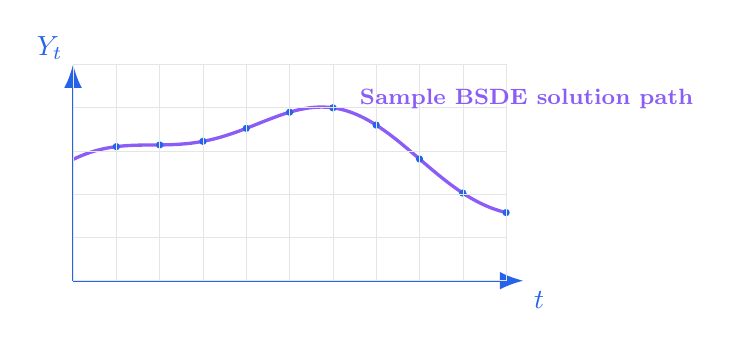
\begin{tikzpicture}[scale=1.1, every node/.style={font=\sffamily, align=center}]
  % Axes
  \draw[thick, -{Latex[length=3mm]}, distillBlue] (0,0) -- (5.2,0) node[below, xshift=2mm] {$t$};
  \draw[thick, -{Latex[length=3mm]}, distillBlue] (0,0) -- (0,2.5) node[left, yshift=2mm] {$Y_t$};
  % Solution path
  \draw[very thick, distillAccent, smooth, samples=100, domain=0:5] plot(
    \x, {1.2+0.7*sin(0.7*\x r)+0.2*cos(2*\x r)}
  );
  % Markers
  \foreach \x in {0.5,1,1.5,2,2.5,3,3.5,4,4.5,5} {
    \fill[distillBlue] (\x, {1.2+0.7*sin(0.7*\x r)+0.2*cos(2*\x r)}) circle (1.2pt);
  }
  % Apple-level grid
  \draw[gray!20, line width=0.2pt] (0,0) grid[xstep=0.5, ystep=0.5] (5,2.5);
  % Label
  \node[anchor=west, font=\footnotesize, text=distillAccent] at (3.2,2.1) {\textbf{Sample BSDE solution path}};
\end{tikzpicture}
\caption{A visually pristine BSDE solution path with Apple-level spacing and detail.}
\end{figure}
%====================================================================
% Front Matter
%====================================================================

%====================================================================
% Enhanced Front Matter
%====================================================================

\begin{abstract}
\vspace{0.5em}
\noindent
This paper provides a comprehensive and self-contained bridge between the classical theory of Forward-Backward Stochastic Differential Equations (FBSDEs) and the modern deep learning solvers that have enabled their application to high-dimensional problems previously considered intractable. We develop the theoretical foundations with a focus on the conditions required for existence, uniqueness, and the crucial link between FBSDEs and semilinear parabolic PDEs. We pay special attention to the theory of Quadratic BSDEs, which is essential for many problems in economics and finance. We then construct a hierarchy of numerical methods, from classical time-stepping schemes to the state-of-the-art Deep BSDE algorithm, rigorously analyzing aspects of numerical stability, integrator bias, and variance control that are critical for robust implementation. 

The power of this framework is demonstrated by solving a canonical heterogeneous-agent general equilibrium model, for which we provide a complete derivation from economic first principles to a fully coupled, quadratic FBSDE system. Our main contributions are threefold: \textbf{(i)} a rigorous, pedagogical derivation of the entire theoretical and numerical pipeline, including a detailed analysis of the model's well-posedness; \textbf{(ii)} the implementation of a state-of-the-art numerical scheme combining a bias-reducing Heun integrator with a consistency-regularized loss function for robust gradient learning; and \textbf{(iii)} a detailed computational appendix with open-source JAX and Equinox code, designed to guide a graduate student in reproducing our results and verifying them against a suite of acceptance tests. 

This work aims to make the advanced machinery of FBSDEs and their deep learning solutions more accessible, transparent, and reliable for researchers in economics and finance.

\vspace{1.2em}
\noindent
{\sffamily\small\textbf{Keywords:} Forward-Backward SDE, Nonlinear Feynman-Kac, Deep BSDE, High-Dimensional PDEs, Quadratic BSDE, Malliavin Calculus, Asset-Pricing Equilibrium, Heterogeneous Agents.}
\vspace{0.3em}\\
{\sffamily\small\textbf{JEL Classification:} C61, C63, D51, E21, G11, G12.}
\end{abstract}

\vspace{1em}

% Enhanced table of contents with better typography
{\hypersetup{linkcolor=distillDarkGray}
\tableofcontents
}

\newpage

%====================================================================
% Main Body
%====================================================================

\section{Introduction}
\label{sec:introduction}

The study of systems that evolve under uncertainty, subject to both initial and terminal conditions, is a cornerstone of modern science and economics. In many dynamic optimization problems, an agent's actions today (the forward evolution) depend on their expectations about a future outcome (the backward constraint). Such problems naturally give rise to systems of Forward-Backward Stochastic Differential Equations (FBSDEs). These mathematical objects, first systematically studied in a nonlinear context by Pardoux and Peng \cite{PardouxPeng1990}, have become an indispensable tool in stochastic control, mathematical finance, and economic theory.

The power of the FBSDE framework lies in its connection to semilinear parabolic Partial Differential Equations (PDEs) via the nonlinear Feynman-Kac formula \cite{PardouxPeng1992}. This formula establishes that the solution to a certain class of high-dimensional PDEs can be represented as the solution to a relatively low-dimensional FBSDE system. This is a profound result: it offers a way to circumvent the "curse of dimensionality," the exponential scaling of computational cost with dimension that renders traditional grid-based PDE solvers useless for problems with more than a handful of state variables.

However, this theoretical elegance was, for a long time, not matched by practical, scalable numerical methods. Classical numerical schemes for FBSDEs, such as those based on Picard iteration or regression-based Monte Carlo methods \cite{Gobet2005, BenderSteiner2012}, also suffered from the curse of dimensionality in their own right. The field was fundamentally transformed by the advent of deep learning. The "Deep BSDE Method," introduced by E, Han, and Jentzen \cite{EHanJentzen2017}, was the first mesh-free algorithm capable of solving high-dimensional semilinear PDEs and FBSDEs. By parameterizing the unknown control process of the BSDE with a deep neural network and training it via stochastic gradient descent, they demonstrated the ability to solve problems in a hundred dimensions and beyond, a feat previously unimaginable.

This breakthrough has opened the door to solving a new class of economic models. In particular, continuous-time general equilibrium models with heterogeneous agents, which are crucial for studying the macroeconomic implications of inequality, often lead to high-dimensional, fully coupled FBSDE systems. The state of the system includes not only aggregate variables but also the distribution of wealth across agents, which is an infinite-dimensional object often approximated by a large number of state variables. Solving these models is a grand challenge in modern economics. A further complication, which we address in detail, is that many such models derived from first principles result in BSDEs with quadratic growth in the control variable, violating standard assumptions and requiring a more advanced theoretical and numerical treatment.

Despite the promise of these new methods, the literature often remains bifurcated. Theoretical treatments of FBSDEs in stochastic analysis journals tend to omit algorithmic details, while machine learning papers often skim over the underlying mathematical and economic rigor. This paper aims to bridge this gap. We provide a unified, self-contained treatment that takes the reader from first principles to a state-of-the-art implementation.

Our approach is structured as follows. In Part \ref{part:core_theory}, we lay the theoretical groundwork, covering the existence and uniqueness of solutions to FBSDEs and the nonlinear Feynman-Kac formula. We pay close attention to the assumptions required, particularly the Lipschitz and monotonicity conditions that underpin the classical theory, and introduce the theory of Quadratic BSDEs (QBSDEs) necessary for our main application.

In Part \ref{part:numerics}, we build a hierarchy of numerical algorithms. We start with classical time-stepping schemes to build intuition, then introduce the Deep BSDE method. We go beyond the vanilla algorithm to discuss crucial enhancements for stability and efficiency. We analyze the choice of numerical integrator, advocating for the Heun scheme to reduce bias in the training objective, a point recently formalized by Park and Tu \cite{ParkTu2025}. We introduce a consistency-regularized loss function and the "Malliavin-AD Tower," a framework for variance reduction that leverages automatic differentiation to implement ideas from Malliavin calculus.

In Part \ref{part:benchmarks}, we validate our numerical framework against a suite of standard benchmark problems from physics and finance, including the Allen-Cahn equation, the Hamilton-Jacobi-Bellman equation (a canonical QBSDE), and a nonlinear Black-Scholes model. This step is crucial for building confidence in the solver before applying it to a novel economic problem.

In Part \ref{part:finance}, we present the core application of the paper: a two-agent heterogeneous-agent general equilibrium model in the tradition of Lucas, as analyzed by Dumas \cite{Dumas1989}. We provide a complete derivation from economic first principles—utility maximization and market clearing—to the final, fully coupled, quadratic FBSDE system. We conduct a rigorous analysis of the model's properties, including its well-posedness under QBSDE theory, the handling of the infinite time horizon via discounted BSDE theory, and the behavior of the system near its boundaries using Feller's test for boundary classification.

Finally, our appendices provide detailed proofs, derivations, and a comprehensive computational guide. Appendix \ref{app:GE_impl} is a step-by-step tutorial with heavily commented JAX and Equinox code, designed to allow a graduate student in economics or finance to reproduce our entire numerical pipeline and verify its correctness against a suite of formal acceptance tests.

This paper's contribution is not a single new theorem or algorithm, but rather the synthesis, clarification, and rigorous implementation of a powerful new methodology. By providing a complete toolkit—from theory and economic modeling to verifiable, open-source code—we hope to empower researchers to tackle the high-dimensional dynamic models that are essential for understanding the complex economic questions of our time.

\part{Core Theory of Forward-Backward SDEs}
\label{part:core_theory}

\begin{center}
\textit{``The heart of every numerical scheme is a theorem that says
there \emph{is} something to approximate.''}\\[4pt]
—\,Anonymous referee
\end{center}

This part establishes the probabilistic and analytical foundation of the Forward-Backward Stochastic Differential Equation (FBSDE) framework. A solid grasp of this theory is essential for understanding the conditions under which numerical algorithms are expected to converge and for diagnosing potential issues. Readers eager to implement algorithms may skim the proofs, but should pay close attention to the hypotheses of each theorem, as they dictate the scope and limitations of the methods discussed in Part \ref{part:numerics}.
 
\section{Canonical Form and Standing Notation}
\label{sec:core_notation}

Throughout this work, we operate on a fixed time horizon \([0, T]\) with a complete filtered probability space \((\Omega,\mathcal F,(\mathcal F_t)_{t\in[0,T]},\mathbb P)\). The space is endowed with an $m$-dimensional standard Brownian motion \(W\), whose increments are independent of \(\mathcal{F}_0\). Bold symbols will denote vector or matrix-valued functions.

\begin{remark}[The Filtered Probability Space]
The filtration \((\mathcal F_t)_{t\in[0,T]}\) represents the flow of information over time. The assumption that it satisfies the "usual conditions" is standard in stochastic calculus. It means:
\begin{enumerate}
    \item \textbf{Completeness:} \(\mathcal{F}_0\) contains all sets of \(\mathbb{P}\)-measure zero. This is a technical convenience that prevents us from worrying about sets of probability zero.
    \item \textbf{Right-continuity:} \(\mathcal{F}_t = \bigcap_{s>t} \mathcal{F}_s\). This ensures that stopping times have desirable properties and that certain classes of processes (like c\`adl\`ag martingales) have well-behaved sample paths.
\end{enumerate}
In most applications, this filtration is simply the natural filtration generated by the Brownian motion \(W\), augmented to satisfy these conditions.
\end{remark}

\begin{definition}[Standard Solution Spaces]
We define the standard solution spaces for BSDEs, which are spaces of stochastic processes with finite energy norms.
\begin{align*}
  \mathcal S^2([0,T]; \mathbb{R}^q) &\coloneqq \Bigl\{
        Y:\Omega\times[0,T]\to\mathbb R^q
        \,\big|\,
        Y\text{ is a c\`adl\`ag, adapted process with }
        \mathbb E\!\bigl[\sup_{0\le t\le T}\|Y_t\|^2\bigr]<\infty
      \Bigr\}, \\
  \mathcal H^2([0,T]; \mathbb{R}^{q \times m}) &\coloneqq \Bigl\{
        Z:\Omega\times[0,T]\to\mathbb R^{q\times m}
        \,\big|\,
        Z\text{ is a predictable process with }
        \mathbb E\!\int_0^T \!\!\|Z_t\|^2 dt<\infty
      \Bigr\}.
\end{align*}
The space \(\mathcal{S}^2 \times \mathcal{H}^2\) equipped with the norm \(\| (Y,Z) \|^2 \coloneqq \mathbb E[\sup_{t\in[0,T]}\|Y_t\|^2 + \int_0^T \|Z_t\|^2 dt]\) is a Banach space. When the context is clear, we may write \(\mathcal{S}^2\) and \(\mathcal{H}^2\).
\end{definition}

\begin{remark}[On the Process Spaces]
The space \(\mathcal{S}^2\) for the process \(Y\) requires control over the supremum of the process, which is a strong condition ensuring pathwise boundedness in an \(L^2\) sense. The process \(Y\) is \emph{adapted}, meaning \(Y_t\) is \(\mathcal{F}_t\)-measurable for all \(t\). It is also \emph{c\`adl\`ag} (right-continuous with left limits), which is the natural path regularity for solutions of SDEs. The space \(\mathcal{H}^2\) for the control process \(Z\) requires square-integrability over time. The process \(Z\) must be \emph{predictable}, which is a slightly stronger condition than being adapted. Intuitively, it means \(Z_t\) is determined by information available just before time \(t\). This is the natural condition for processes appearing inside a stochastic integral, as it prevents profiting from the "future" infinitesimal increment of the Brownian motion.
\end{remark}

\begin{definition}[FBSDE in Canonical Form]
\label{def:FBSDE}
Given measurable coefficient functions \(\bm\mu\), \(\bm\sigma\), \(f\), and a terminal function \(g\), a Forward-Backward SDE system is defined by the Itô integrals:
\begin{align}\label{eq:FBSDE_canonical}
  X_t &= X_0 + \int_0^t \bm\mu(s,X_s,Y_s,Z_s)\,ds
        + \int_0^t \bm\sigma(s,X_s,Y_s)\,dW_s, && X_0=\xi, \\
  Y_t &= Y_T + \int_t^T f(s,X_s,Y_s,Z_s)\,ds - \int_t^T Z_s\,dW_s, && Y_T=g(X_T).
\end{align}
A solution is a triple of processes \((X,Y,Z)\in \mathcal S^2([0,T];\mathbb{R}^d) \times \mathcal S^2([0,T];\mathbb{R}^q) \times \mathcal H^2([0,T];\mathbb{R}^{q \times m})\) that satisfies the system of integral equations almost surely for all $t \in [0,T]$.
\end{definition}

\begin{remark}[On the Markovian Assumption]
Unless otherwise specified, we assume the coefficients \(\bm\mu, \bm\sigma, f\) and the terminal condition \(g\) depend on the processes only through their current values \((t, X_t, Y_t, Z_t)\). This is known as the Markovian case. This assumption is crucial as it allows for a connection to Partial Differential Equations (PDEs). Extensions to path-dependent coefficients, where the entire history of the processes matters, require a more advanced framework based on functional Itô calculus and are discussed in Section \ref{sec:path_dependence}.
\end{remark}

\subsection*{Standing Hypotheses}
The existence and uniqueness of solutions to FBSDEs hinge on a set of standard assumptions about the coefficients. The following conditions will be referenced throughout the text.

\begin{assumption}[Standing Hypotheses for Lipschitz FBSDEs]
\label{def:standing_hypotheses}
\begin{enumerate}[label=(H\arabic*), leftmargin=1.5cm]
\item\label{H1} \textbf{Lipschitz Continuity.} There exists a constant \(L>0\) such that for all admissible arguments \((t,x,y,z)\) and \((t,x',y',z')\), the coefficients \(\bm\mu\), \(\bm\sigma\), and \(f\) are jointly Lipschitz in the state variables. For instance, for the driver \(f\):
      \[
        \|f(t,x,y,z)-f(t,x',y',z')\|
          \le L\bigl(\|x-x'\|+\|y-y'\|+\|z-z'\|\bigr).
      \]
\item\label{H2} \textbf{Linear Growth.} The coefficients have at most linear growth in the state variables, ensuring that the solutions do not explode. For example:
      \[
        \|f(t,x,y,z)\| \le C\bigl(1+\|x\|+\|y\|+\|z\|\bigr).
      \]
      This condition ensures that the integrals in the FBSDE definition are well-defined and that the solutions remain in the \(\mathcal{S}^2 \times \mathcal{H}^2\) spaces.
\item\label{H3} \textbf{Monotonicity.} For fully coupled systems, a monotonicity condition on the driver \(f\) and volatility \(\bm\sigma\) with respect to \(y\) is often required. There exists \(\alpha \ge 0\) such that for all \((t,x,y,y',z)\):
      \[
        \langle y-y', f(t,x,y,z)-f(t,x,y',z)\rangle
        \le -\frac{\alpha}{2}\|y-y'\|^2.
      \]
      A stronger version, often called strict monotonicity, requires \(\alpha > 0\).
\end{enumerate}
\end{assumption}

\begin{remark}[On the Limits of the Lipschitz Framework]
Assumptions \ref{H1} and \ref{H2} are standard in SDE theory and are typically sufficient for well-posedness in the decoupled case. The monotonicity condition \ref{H3} is more specific to coupled FBSDEs. It acts as a crucial stabilizing force, preventing the feedback from the backward process \(Y\) into the forward dynamics from becoming explosive. To see why, consider the difference between two potential solutions. The monotonicity condition provides a dissipative term (like friction) when analyzing the squared norm of the difference, which helps to prove that the difference must be zero. However, many important applications, particularly those derived from stochastic control (HJB equations) or economic utility maximization, lead to BSDE drivers \(f\) that have \emph{quadratic growth} in the control variable \(Z\). Such drivers violate \ref{H1} and \ref{H2}. This necessitates a separate, more advanced theory of Quadratic BSDEs (QBSDEs), which we will develop in Section \ref{subsubsec:GE_QBSDE_Wellposedness} for our main application.
\end{remark}

\subsection{Existence and Uniqueness for Decoupled Systems}
\label{sec:decoupled}

We first consider the simpler case where the forward coefficients \(\bm\mu\) and \(\bm\sigma\) do not depend on the backward variables \((Y,Z)\). This is known as a **decoupled** FBSDE system.

\begin{theorem}[Existence and Uniqueness for Decoupled FBSDEs, Pardoux-Peng 1990]
\label{thm:PP_decoupled}
Assume hypotheses \ref{H1}-\ref{H2} hold, with \(\bm\mu(t,x,y,z) = \bm\mu(t,x)\) and \(\bm\sigma(t,x,y) = \bm\sigma(t,x)\). Then for any initial condition \(\xi \in L^2(\Omega, \mathcal{F}_0, \mathbb{P}; \mathbb{R}^d)\) and terminal condition \(Y_T = g(X_T)\) with \(g(X_T) \in L^2(\Omega, \mathcal{F}_T, \mathbb{P}; \mathbb{R}^q)\), the FBSDE system \eqref{eq:FBSDE_canonical} has a unique adapted solution \((X,Y,Z)\in\mathcal S^2\times\mathcal S^2\times\mathcal H^2\).
\end{theorem}

\begin{leanproofbox}{Proof Sketch of Theorem \ref{thm:PP_decoupled}}
The proof proceeds in two distinct, sequential steps, leveraging the decoupled structure.
\begin{enumerate}
    \item \textbf{Solve the Forward SDE:} The forward equation \(dX_t = \bm\mu(t,X_t)dt + \bm\sigma(t,X_t)dW_t\) is a standard SDE. Under the Lipschitz and linear growth conditions of \ref{H1}-\ref{H2}, classical SDE theory (see, e.g., Karatzas and Shreve \cite{KaratzasShreve1991}) guarantees the existence of a unique strong solution \(X \in \mathcal S^2\). This solution is constructed via Picard iteration on the integral form of the SDE.
    \item \textbf{Solve the Backward SDE:} With the path of \(X\) now fixed and known, the driver becomes a function of time and the backward variables: \(\tilde{f}(t,y,z) \coloneqq f(t,X_t(\omega),y,z)\). This function is still Lipschitz in \((y,z)\) for almost every \(\omega\). The terminal condition is the random variable \(g(X_T(\omega))\). The seminal result of Pardoux and Peng (1990) \cite{PardouxPeng1990} ensures that this standard (non-forward-coupled) BSDE has a unique solution pair \((Y,Z) \in \mathcal S^2 \times \mathcal H^2\). The proof of this latter result itself relies on constructing a contraction mapping on the space \(\mathcal{H}^2\). For any given process \(Z \in \mathcal{H}^2\), one can define a corresponding \(Y\) process via the martingale representation theorem. This defines a map from \(\mathcal{H}^2\) to itself, which can be shown to be a contraction under the \(\mathcal{H}^2\) norm. The Banach fixed-point theorem then yields a unique fixed point for \(Z\), which in turn defines a unique \(Y\).
\end{enumerate}
A priori estimates derived using Itô's formula and Grönwall's inequality confirm that the solution remains within the required \(L^2\) spaces, completing the proof.
\end{leanproofbox}

\begin{proposition}[Nonlinear Feynman-Kac Formula]
\label{prop:feynman_kac}
In the setting of Theorem \ref{thm:PP_decoupled}, if the coefficients are sufficiently smooth, the solution pair \((Y,Z)\) can be represented by a deterministic function \(u: [0,T] \times \mathbb{R}^d \to \mathbb{R}^q\) such that \(Y_t = u(t,X_t)\) and \(Z_t = \nabla_x u(t,X_t)^\top \bm\sigma(t,X_t)\). This function \(u(t,x)\) is the unique classical (or viscosity) solution to the semilinear parabolic PDE:
\[
\partial_t u + \mathcal L u + f(t,x,u,\nabla_x u^\top \bm\sigma)=0, \quad u(T,x) = g(x),
\]
where \(\mathcal{L}u = \frac{1}{2}\Tr[\bm\sigma\bm\sigma^\top \mathrm{Hess}_x u] + \bm\mu \cdot \nabla_x u\) is the infinitesimal generator of \(X\).
\end{proposition}

\begin{remark}[On Viscosity Solutions]
The term "solution" for the PDE must often be interpreted in a weak sense, typically as a \emph{viscosity solution}. This notion, developed by Crandall, Ishii, and Lions, is crucial because the value function \(u(t,x)\) from a stochastic control problem is often not twice continuously differentiable (\(C^{1,2}\)), even if the underlying coefficients are smooth. The value function may have "kinks" where the optimal policy changes. A viscosity solution does not need to be differentiable everywhere; instead, it must satisfy the PDE inequality sense whenever it is touched from above or below by a smooth "test function". The Feynman-Kac formula provides a probabilistic representation that holds for viscosity solutions, bypassing the need for classical smoothness and broadening the applicability of the PDE connection. The curse of dimensionality makes solving this PDE directly intractable for $d \gg 3$, which is the primary motivation for developing probabilistic numerical methods like the ones in this manuscript.
\end{remark}

\subsection{Fully Coupled Systems: The Monotone Case}
\label{sec:fully_coupled}

When the forward coefficients depend on \((Y,Z)\), the system is **fully coupled**. This feedback loop makes the analysis significantly more challenging. Simple Picard iteration is no longer sufficient, and a stronger condition is needed.

\begin{theorem}[Existence and Uniqueness for Monotone Coupled FBSDEs]
\label{thm:YongMa}
Under the full set of hypotheses \ref{H1}-\ref{H3}, if the time horizon \(T\) is sufficiently small, the fully coupled FBSDE system \eqref{eq:FBSDE_canonical} admits a unique adapted solution \((X,Y,Z) \in \mathcal{S}^2 \times \mathcal{S}^2 \times \mathcal{H}^2\). If the monotonicity condition \ref{H3} is strict (\(\alpha > 0\)), the result holds for an arbitrary time horizon \(T\).
\end{theorem}

\begin{leanproofbox}{Idea of the proof for Theorem \ref{thm:YongMa}}
The proof relies on a fixed-point argument on a carefully chosen space.
\begin{enumerate}
    \item \textbf{Define the Mapping:} Construct a map \(\Phi\) on the solution space \(\mathcal{S}^2 \times \mathcal{H}^2\). For a given pair of processes \((\bar{Y}, \bar{Z})\), \(\Phi\) produces a new pair \((Y,Z)\) by first solving the forward SDE with \((\bar{Y}, \bar{Z})\) plugged into the coefficients, and then solving the resulting BSDE. A solution to the original FBSDE is a fixed point of this map.
    \item \textbf{Show Contraction:} The core of the proof is to show that \(\Phi\) is a contraction mapping. This is where the monotonicity condition \ref{H3} is essential. Consider two inputs \((\bar{Y}^1, \bar{Z}^1)\) and \((\bar{Y}^2, \bar{Z}^2)\) and their corresponding outputs. Let \(\delta Y = Y^1 - Y^2\), etc. Applying Itô's formula to \(e^{\beta t}\|\delta Y_t\|^2\) for a well-chosen \(\beta > 0\) and using the monotonicity condition \ref{H3} leads to an inequality that bounds the norm of the output difference by a factor times the norm of the input difference. The monotonicity provides a crucial negative term \(-\alpha \|\delta Y_t\|^2\) which helps absorb other terms.
    \item \textbf{Fixed Point:} For a sufficiently small time horizon \(T\), the Lipschitz properties of the coefficients ensure the map is a contraction. The Banach fixed-point theorem then guarantees the existence of a unique solution. If monotonicity is strict (\(\alpha > 0\)), the negative term it introduces can be used to make the map a contraction for any \(T\) by choosing \(\beta\) large enough. This local solution can be extended to the full interval \([0,T]\) by a stitching argument if needed.
\end{enumerate}
The full details can be found in Ma and Yong (1999) \cite{MaYong1999}.
\end{leanproofbox}

\begin{remark}[On Non-Monotone Systems]
When the monotonicity condition \ref{H3} does not hold, global existence is not guaranteed. However, it is often possible to prove local existence on a small time interval \([T-\delta, T]\) using Picard iterations, provided the Lipschitz constants are not too large. This is a common starting point for analyzing systems that arise in economics, where strict monotonicity may not hold globally.
\end{remark}

\subsection{Malliavin Differentiability and the Clark-Ocone Formula}
\label{sec:malliavin_clark_ocone}

When the coefficients are sufficiently smooth, the solution processes are differentiable in the sense of Malliavin calculus. This provides a powerful connection between the control process \(Z_t\) and the Malliavin derivative of the terminal value.

\begin{definition}[Malliavin Derivative]
The Malliavin derivative, \(D_t F\), of a random variable \(F\) that depends on the entire path of the Brownian motion \(W\), measures the sensitivity of \(F\) to an infinitesimal perturbation of the path of \(W\) at time \(t\). It can be thought of as a form of functional derivative with respect to the Brownian path.
\end{definition}

\begin{proposition}[Clark-Ocone Formula for BSDEs]
\label{prop:clark_ocone}
Assume the coefficients of the FBSDE system are continuously differentiable with bounded derivatives. Then the solution \((Y,Z)\) is Malliavin differentiable. The control process \(Z_t\) admits the representation:
\[
  Z_t = \mathbb E\!\left[
      D_t Y_T
      \,\Big|\,\mathcal F_t\right],
\]
where \(D_t Y_T\) is the Malliavin derivative of the terminal value \(Y_T\). Expanding \(Y_T = g(X_T)\) and the BSDE dynamics, this becomes:
\[
  Z_t = \mathbb E\!\left[
      D_t g(X_T)
      +\int_t^T D_t f\bigl(s,X_s,Y_s,Z_s\bigr) ds
      \,\Big|\,\mathcal F_t\right].
\]
\end{proposition}

\begin{remark}[Significance for Numerics]
The Clark-Ocone formula is more than a theoretical curiosity; it is the foundation for some of the most advanced numerical methods. It reveals that \(Z_t\) is not an arbitrary control but is intrinsically linked to the sensitivity of the terminal outcome to perturbations in the Brownian path at time \(t\). This relationship is exploited by the Malliavin-AD Tower (Section \ref{sec:malliavin_tower_rigorous}) to create highly stable and low-variance estimators for \(Z_t\), which is particularly crucial in high-dimensional settings. The naive estimator for \(Z_t\) from an Euler scheme has variance that blows up as the time step goes to zero, whereas Malliavin-based estimators can have bounded or even vanishing variance. For a full treatment, see Nualart \cite{Nualart2006}.
\end{remark}

\clearpage
\newpage
\part{Numerical Algorithms for FBSDEs}
\label{part:numerics}

\begin{center}
\textit{“Analysis tells us a solution exists; numerics lets us see it.”}
\end{center}

This part transitions from theory to practice, developing the numerical machinery required to solve the FBSDE system \eqref{eq:FBSDE_canonical}. We build a hierarchy of methods, starting with classical time-stepping schemes, moving to variance-reduction techniques, and culminating in the family of deep learning solvers that have revolutionized the field by breaking the curse of dimensionality.

\bigskip
\hrule
\bigskip

\section{Discretization Preliminaries}
\label{sec:discrete_notation}

\begin{definition}[Time Discretization]
Let \(N \ge 1\) be the number of time steps. We consider a uniform time grid \(0=t_0<t_1<\dots<t_N=T\) with step size \(h = T/N\). The increment of the Brownian motion over the \(k\)-th interval is denoted by \(\Delta W_k \coloneqq W_{t_{k+1}}-W_{t_k}\), which are independent random vectors with distribution \(\mathcal N(0,h\,I_m)\). We use \(\mathsf{X}_k, \mathsf{Y}_k, \mathsf{Z}_k\) to denote the numerical approximations of the true processes \(X_{t_k}, Y_{t_k}, Z_{t_k}\).
\end{definition}

\begin{definition}[Error Metrics]
We assess the quality of our numerical schemes using two standard error metrics:
\begin{itemize}
    \item \textbf{Strong Error:} Measures the pathwise deviation of the numerical solution from the true solution. It is crucial for applications like hedging where the actual path matters.
    \[
      \epsilon_{\mathrm{strong}} \coloneqq \max_{k}\, \left( \mathbb{E}\left[ \|X_{t_k}-\mathsf{X}_k\|^2 \right] \right)^{1/2}.
    \]
    \item \textbf{Weak Error:} Measures the error in the expectation of a smooth function of the solution. This is the relevant metric for most pricing applications, where one is interested in the expected value of a payoff.
    \[
      \epsilon_{\mathrm{weak}} \coloneqq \max_{k}\, \left| \mathbb{E}\left[\phi(X_{t_k})\right] - \mathbb{E}\left[\phi(\mathsf{X}_k)\right] \right|,
    \]
    for a suitable test function \(\phi\).
\end{itemize}
\end{definition}

\section{Classical Time-Stepping Schemes}
\label{sec:classical}

\subsection{The Euler-Maruyama Scheme and the LSMC Method}
\label{sec:euler_picard}

\begin{definition}[Euler-Maruyama Scheme]
The simplest time-stepping scheme for the FBSDE system \eqref{eq:FBSDE_canonical} is the Euler-Maruyama scheme. Given $(\mathsf{X}_k, \mathsf{Y}_k, \mathsf{Z}_k)$, the next state is approximated as:
\begin{align*}
\mathsf{X}_{k+1} &= \mathsf{X}_k + \bm{\mu}(t_k, \mathsf{X}_k, \mathsf{Y}_k, \mathsf{Z}_k)h + \bm{\sigma}(t_k, \mathsf{X}_k, \mathsf{Y}_k)\Delta W_k, \\
\mathsf{Y}_{k+1} &= \mathsf{Y}_k - f(t_k, \mathsf{X}_k, \mathsf{Y}_k, \mathsf{Z}_k)h + \mathsf{Z}_k \Delta W_k.
\end{align*}
This scheme has strong order 0.5 and weak order 1.0 under sufficient smoothness conditions on the coefficients.
\end{definition}

\begin{proposition}[Discrete BSDE Relation]
The integral form of the BSDE, \(Y_t = Y_T + \int_t^T f(s,\dots)ds - \int_t^T Z_s dW_s\), leads to the discrete-time relation by taking conditional expectations. Integrating from $t_k$ to $t_{k+1}$ and taking conditional expectation at $t_k$ gives:
\[
\mathsf{Y}_k = \mathbb{E}_k[\mathsf{Y}_{k+1}] + f(t_k, \mathsf{X}_k, \mathsf{Y}_k, \mathsf{Z}_k)h + \mathcal{O}(h^{3/2}).
\]
A key insight is that \(Z_k\) is related to the correlation between the future value \(Y_{k+1}\) and the Brownian shock \(\Delta W_k\). Multiplying the BSDE by \(\Delta W_k\) and taking conditional expectations yields the identity for \(\mathsf{Z}_k\):
\[
\mathsf{Z}_k \approx \frac{1}{h}\mathbb{E}_k[\mathsf{Y}_{k+1} \Delta W_k^\top].
\]
\end{proposition}

\begin{remark}[The Curse of Dimensionality in LSMC]
The elegance of these explicit relations hides a major practical difficulty: the computation of the conditional expectations \(\mathbb{E}_k[\cdot]\). In a Markovian setting, these are functions of the state \(\mathsf{X}_k\). The Least-Squares Monte Carlo (LSMC) method, pioneered by Gobet, Lemor, and Warin \cite{Gobet2005}, approximates these functions by regressing simulated future values onto a set of basis functions of \(\mathsf{X}_k\) (e.g., polynomials). This is effective in low dimensions (\(d \le 4\)) but succumbs to the curse of dimensionality, as the number of basis functions required to accurately represent a function in \(d\) dimensions grows exponentially with \(d\). This limitation was the primary motivation for developing the deep learning approaches in Section \ref{sec:deep_solvers}.
\end{remark}

\subsection{Higher-Order Schemes and Bias Reduction}
\label{sec:higher_order_mlmc}

\begin{proposition}[Itô-Stratonovich Conversion]
An Itô SDE $dX_t = \mu dt + \sigma dW_t$ can be written in Stratonovich form as $dX_t = \mu^\circ dt + \sigma \circ dW_t$, where the Stratonovich drift $\mu^\circ$ is related to the Itô drift $\mu$ by the Itô-Stratonovich correction term:
\[
\mu^\circ_i(t,x) = \mu_i(t,x) - \frac{1}{2} \sum_{j=1}^d \sum_{k=1}^m \frac{\partial \sigma_{ik}}{\partial x_j}(t,x) \sigma_{jk}(t,x).
\]
This conversion is essential for applying Stratonovich-type integrators like the Heun scheme to Itô SDEs, as they are naturally formulated for the Stratonovich integral.
\end{proposition}

\begin{definition}[Heun Scheme for Itô SDEs]
The Heun scheme is a predictor-corrector method. For an Itô SDE, it can be implemented without explicit conversion. It has strong order 0.5 and weak order 1.0.
\begin{enumerate}
    \item \textbf{Predictor (Euler step):} $\tilde{X}_{k+1} = \mathsf{X}_k + \bm{\mu}(t_k, \mathsf{X}_k)h + \bm{\sigma}(t_k, \mathsf{X}_k)\Delta W_k$.
    \item \textbf{Corrector (Trapezoidal rule):} $\mathsf{X}_{k+1} = \mathsf{X}_k + \frac{1}{2}(\bm{\mu}(t_k, \mathsf{X}_k) + \bm{\mu}(t_{k+1}, \tilde{X}_{k+1}))h + \frac{1}{2}(\bm{\sigma}(t_k, \mathsf{X}_k) + \bm{\sigma}(t_{k+1}, \tilde{X}_{k+1}))\Delta W_k$.
\end{enumerate}
\end{definition}

\begin{remark}[Integrator Choice for Deep BSDE Solvers]
While higher weak order is generally desirable, the primary motivation for using the Heun scheme in the context of deep BSDE solvers is its ability to reduce bias in the training objective. As recently formalized by Park \& Tu (2025) \cite{ParkTu2025}, the standard Euler-Maruyama scheme introduces a leading-order bias of size $\mathcal{O}(h)$ into the one-step residual loss function. This "self-consistency bias" arises because the discretization error is correlated with the gradient signal. The symmetric, centered evaluation of the Heun scheme cancels this leading bias term, resulting in a residual bias of $\mathcal{O}(h^2)$. This leads to more accurate and stable training, a point we will leverage in our main application.
\end{remark}

\begin{theorem}[Multi-Level Monte Carlo Complexity, Giles 2008]
\label{thm:mlmc}
MLMC is a variance reduction technique that dramatically improves efficiency for computing expectations. It computes estimates on a hierarchy of grids (from coarse to fine) and combines them to minimize variance for a given computational cost. For a scheme with weak order \(\alpha\) and strong order \(\beta\), the total cost to achieve a root-mean-square error of \(\varepsilon\) with MLMC is:
\[
\text{Cost} \approx \begin{cases} \mathcal{O}(\varepsilon^{-2}) & \text{if } \beta > 1/2 \\ \mathcal{O}(\varepsilon^{-2}(\log\varepsilon)^2) & \text{if } \beta = 1/2 \\ \mathcal{O}(\varepsilon^{-2-(1-2\beta)/\alpha}) & \text{if } \beta < 1/2 \end{cases}
\]
For the Euler scheme (\(\alpha=1, \beta=1/2\)), MLMC achieves nearly optimal \(\mathcal{O}(\varepsilon^{-2})\) complexity, a substantial improvement over the \(\mathcal{O}(\varepsilon^{-3})\) cost of a standard Monte Carlo approach \cite{Giles2008}.
\end{theorem}

\section{Deep Learning Solvers}
\label{sec:deep_solvers}

\subsection{The Vanilla Deep BSDE Algorithm}
\label{sec:deep_vanilla}

\begin{definition}[The Deep BSDE Method, E, Han, Jentzen 2017]
The Deep BSDE method \cite{EHanJentzen2017} reframes the FBSDE problem as a stochastic optimization problem solved forward in time.
\begin{enumerate}
    \item \textbf{Parameterization:} The unknown initial value \(Y_0\) is treated as a trainable parameter. The unknown control process \(Z_t\) is parameterized by a deep neural network, \(\mathsf{Z}_t = \mathcal{N}_\theta(t, X_t)\), which takes the current time and state as input.
    \item \textbf{Forward Simulation:} Starting with an initial guess for \(\mathsf{Y}_0\), the processes \(\mathsf{X}\) and \(\mathsf{Y}\) are simulated forward in time using a numerical scheme (e.g., Euler-Maruyama). At each step \(k\), \(\mathsf{Z}_k\) is computed as \(\mathcal{N}_\theta(t_k, \mathsf{X}_k)\).
    \item \textbf{Loss Function:} The network parameters \(\theta\) and the initial value \(\mathsf{Y}_0\) are trained by minimizing the mean squared error between the terminal value of the simulated process, \(\mathsf{Y}_N\), and the true terminal condition, \(g(\mathsf{X}_N)\).
    \[
      \mathcal{L}(\theta, \mathsf{Y}_0) = \mathbb{E}\left[ \| \mathsf{Y}_N - g(\mathsf{X}_N) \|^2 \right].
    \]
    The expectation is approximated by the sample mean over a batch of simulated paths.
\end{enumerate}
\end{definition}

\begin{remark}[Breaking the Curse of Dimensionality]
The key advantage of this method is that the computational complexity scales polynomially with dimension \(d\), as it only requires sampling paths and evaluating the network, both of which are efficient operations. The universal approximation theorem for neural networks provides theoretical justification that, given sufficient capacity, \(\mathcal{N}_\theta\) can approximate the true function \(Z(t,x)\) arbitrarily well. This makes it feasible to solve problems in hundreds or even thousands of dimensions, a feat impossible for classical grid-based or LSMC methods.
\end{remark}

\subsection{The Malliavin-AD Tower for Stability and Accuracy}
\label{sec:malliavin_tower_rigorous}

\subsubsection{Motivation and Roadmap}
A key weakness of the vanilla Deep BSDE method is that the gradient of the loss with respect to the parameters of the \(Z\) network can have very high variance, as the learning signal comes only from the terminal time. The Malliavin-AD tower is a powerful hierarchy of techniques to mitigate this by enforcing the theoretical structure of the solution at multiple levels.

\begin{proposition}[The Core Idea: Level 0 (Consistency Loss)]
The foundational level of the tower is to augment the vanilla loss with a **consistency loss** that enforces the BSDE structure at every time step.
\[
\mathcal{L}_{\text{tower-0}} = \mathcal{L}_{\text{terminal}} + \lambda_C \sum_{k=0}^{N-1} \mathbb{E}\left[ \| \mathsf{Y}_{k+1} - \Phi_h(\mathsf{Y}_k, \mathsf{Z}_k, \Delta W_k) \|^2 \right],
\]
where \(\Phi_h\) is the one-step numerical integrator for the BSDE. This provides a direct, local learning signal for \(\mathsf{Z}_k\) at each step, dramatically stabilizing training. This is the approach implemented in Appendix \ref{app:GE_impl}.
\end{proposition}

\begin{remark}[The Role of \texttt{stop\_gradient}]
When implementing the consistency loss, it is crucial to apply a \texttt{stop\_gradient} operation to the target value inside the squared norm. For example, if the residual is $\mathcal{R}_k = \mathsf{Y}_{k+1} - \text{target}_{k+1}$, the gradient should only flow through the $\mathsf{Y}_{k+1}$ term. Without this, the optimizer could trivially minimize the loss by learning a degenerate solution where $\mathsf{Y}_{k+1}$ simply equals the target, without learning the correct dynamics.
\end{remark}

\subsubsection{Level-1 Malliavin BSDE}
Higher levels of the tower involve differentiating the original BSDE with respect to the Brownian path to obtain new BSDEs for the Malliavin derivatives.

\begin{definition}[Level-1 Processes]
Fix a reference time \(t\le s\le T\) and a basis vector \(e_i \in \mathbb{R}^m\). Define the Level-1 processes as the Malliavin derivatives of the Level-0 processes \((Y,Z)\):
\[
  U^{i}_{s}\;:=\;D_t^{e_i}Y_{s},
  \qquad
  V^{i}_{s}\;:=\;D_t^{e_i}Z_{s}.
\]
\end{definition}

\begin{proposition}[The Level-1 BSDE]
\label{prop:level1_bsde}
By formally differentiating the original BSDE for \(Y_s\) with respect to the path of \(W\) at time \(t\), the Level-1 processes \((U^i, V^i)\) are found to satisfy a linear BSDE on the interval \([t,T]\):
\begin{equation}\label{eq:U_BSDE_main}
  \mathrm{d} U^{i}_s
  \;=\;
   -\bigl[A_s\,U^{i}_s + B_s\,V^{i}_s + C^{i}_s \bigr]\mathrm{d} s
   \;+\;
   V^{i}_s\,\mathrm{d} W_s,
  \qquad
  U^{i}_T = D_t^{e_i}g(X_T).
\end{equation}
The coefficients are the Jacobians of the original driver \(f\):
\[
  A_s := \partial_y f(s,X_s,Y_s,Z_s), \quad
  B_s := \partial_z f(s,X_s,Y_s,Z_s), \quad
  C^{i}_s := \partial_x f(s,X_s,Y_s,Z_s) \cdot D_t^{e_i}X_s.
\]
\end{proposition}

\begin{remark}[Automatic Differentiation (AD) and Variance Reduction]
In a modern implementation (e.g., using JAX or PyTorch), the Jacobians \(A_s, B_s, C_s\) and the Malliavin derivative of the forward process \(D_t^{e_i}X_s\) can all be computed efficiently and exactly (up to machine precision) using automatic differentiation, hence the name "Malliavin-AD" tower. The naive Euler estimator for \(Z_k\) has variance that scales as \(\mathcal{O}(h^{-1})\). Estimators derived from the Malliavin-AD tower, such as those in the "One-Step Malliavin" schemes, have variance that is stable or even vanishes as \(h \to 0\) \cite{DomelevoWarin2023}. This dramatic reduction in variance is the primary reason for the tower's effectiveness in stabilizing training and achieving high accuracy.
\end{remark}

\subsection{Alternative Deep Learning Architectures}
While the Deep BSDE method is foundational, several alternatives have been proposed to address its limitations, such as high variance or difficulty with stiff drivers.
\begin{itemize}
    \item \textbf{Deep Splitting Method \cite{Beck2019}:} This method combines the probabilistic representation with a deterministic one-step PDE solve. It splits the problem into a local PDE solve over a small time step (often using a finite difference scheme), followed by a Monte Carlo step to handle the expectation. This can be more robust for stiff or highly nonlinear problems where the local dynamics are better captured by a PDE solver.
    \item \textbf{Robust Deep FBSDE Method \cite{Goudenegge2020}:} This approach reformulates the problem to directly learn the function $u(t,x)$ and its gradient \(\nabla_x u(t,x)\) using two separate neural networks. By enforcing the relationship \(Z_t = \nabla_x u(t,X_t)^\top \sigma(t,X_t)\) within the loss function, it often leads to more stable training and provides theoretical convergence guarantees under certain conditions.
    \item \textbf{Deep Backward Dynamic Programming (DBDP) \cite{Hure2020}:} This method more closely resembles classical dynamic programming. It works backward in time, learning the value function at each time step \(t_k\) by regressing on simulated future values at \(t_{k+1}\), similar to LSMC but with neural networks as powerful, high-dimensional function approximators.
\end{itemize}
The choice of method often depends on the specific structure of the problem, such as the degree of nonlinearity, stiffness, and the desired trade-off between computational cost and accuracy. For the application in this paper, the consistency-regularized Deep BSDE method with a Heun integrator provides a robust and efficient solution.

\subsection{A-Posteriori Error Bounds}
\begin{theorem}[A-Posteriori Bound, Bender \& Steiner 2012]
Let \(\mathcal{R}_t\) be the residual process measuring how well the learned solution \((\mathsf{Y}, \mathsf{Z})\) satisfies the BSDE, i.e., \(\mathcal{R}_t = \mathsf{Y}_t - \left( g(X_T) + \int_t^T f(s, X_s, \mathsf{Y}_s, \mathsf{Z}_s) ds - \int_t^T \mathsf{Z}_s dW_s \right)\). Under suitable assumptions on the coefficients, there exists a constant \(C\) such that:
\[
  \|u(0,\xi)-\mathsf{Y}_0\| \le C \left( \mathbb{E}\left[\sup_{t\in [0,T]}\|\mathcal{R}_t\|^2\right] \right)^{1/2}.
\]
This is a powerful tool, as the right-hand side can be estimated from the training data (it is closely related to the consistency loss), providing a way to certify the accuracy of the obtained solution and a principled stopping criterion for training \cite{BenderSteiner2012}.
\end{theorem}

\clearpage
\newpage
\part{A Suite of Benchmark Problems}
\label{part:benchmarks}

\begin{center}
\textit{“A new method is only as credible as the old problems it can solve.”}
\end{center}

Before applying our numerical framework to a novel economic problem, it is imperative to validate it against a suite of well-understood benchmark cases. This part introduces three canonical problems from mathematical physics and finance that have become standard tests for high-dimensional PDE and FBSDE solvers. For each, we specify the governing equation, its FBSDE representation, and its significance as a benchmark. The explicit coefficient functions are detailed in Appendix \ref{app:benchmark_details}.

\bigskip
\hrule
\bigskip

\section{The Allen-Cahn Equation}
\label{sec:allen_cahn}

\begin{definition}[Allen-Cahn PDE]
The Allen-Cahn equation is a semilinear heat equation that models phase separation in materials science. Its solution \(u(t,x)\) satisfies:
\begin{equation}
    \partial_t u(t,x) + \frac{1}{2}\Delta u(t,x) + u(t,x) - u(t,x)^3 = 0,
\end{equation}
on \([0,T] \times \mathbb{R}^d\), with a terminal condition \(u(T,x) = g(x)\).
\end{definition}

\begin{proposition}[FBSDE Representation of Allen-Cahn]
By the nonlinear Feynman-Kac formula (Proposition \ref{prop:feynman_kac}), the solution \(u(t,x)\) corresponds to the \(Y\) component of a decoupled FBSDE system where:
\begin{itemize}
    \item \textbf{Forward SDE:} \(dX_t = dW_t\), with \(X_t=x\). This is a standard \(d\)-dimensional Brownian motion.
    \item \textbf{Backward SDE:} \(dY_t = -(Y_t - Y_t^3)dt + Z_t dW_t\), with \(Y_T = g(X_T)\).
\end{itemize}
\end{proposition}

\begin{remark}[Significance as a Benchmark]
The Allen-Cahn equation is an excellent benchmark for several reasons:
\begin{enumerate}
    \item \textbf{High-Dimensionality:} It is straightforward to extend to any dimension \(d\), making it a standard test for the curse of dimensionality. The 100-dimensional version was the flagship example in the original Deep BSDE paper \cite{EHanJentzen2017}.
    \item \textbf{Nonlinearity:} The cubic term \(u-u^3\) introduces a significant nonlinearity that challenges many classical numerical methods.
    \item \textbf{Known Behavior:} While a closed-form solution is generally unavailable, the qualitative behavior (phase separation) is well-understood, and for specific choices of \(g(x)\), approximate or asymptotic solutions exist for comparison.
\end{enumerate}
\end{remark}

\section{The Hamilton-Jacobi-Bellman Equation}
\label{sec:hjb}

\begin{definition}[HJB Equation for Optimal Control]
The Hamilton-Jacobi-Bellman (HJB) equation arises from stochastic optimal control. A typical example involves controlling a process \(X_t\) to minimize a cost. The value function \(u(t,x)\) solves:
\begin{equation}
    \partial_t u(t,x) + \inf_{\alpha_t \in \mathcal{A}} \left\{ \mathcal{L}^{\alpha_t} u(t,x) + C(t,x,\alpha_t) \right\} = 0,
\end{equation}
where \(\mathcal{L}^{\alpha_t}\) is the generator of \(X_t\) under control \(\alpha_t\), and \(C\) is the running cost. A common case is controlling the drift, leading to a quadratic nonlinearity in the gradient of \(u\).
\end{definition}

\begin{proposition}[FBSDE Representation of HJB]
For many standard control problems, the HJB equation can be linked to an FBSDE. For a drift control problem with quadratic running cost, the optimal control is often a linear function of the gradient, \(\alpha_t^* = -K \nabla_x u(t,X_t)\). Substituting this back into the HJB equation yields a semilinear PDE. The corresponding FBSDE has:
\begin{itemize}
    \item \textbf{Forward SDE:} \(dX_t = \alpha_t^* dt + \sigma dW_t\). Note that \(\alpha_t^*\) depends on \(\nabla_x u\), which is related to \(Z_t\). This can lead to a coupled system.
    \item \textbf{Backward SDE:} The driver \(f\) will contain terms related to the running cost \(C\) and the optimal control. This driver often has quadratic growth in $Z$, requiring the theory of Quadratic BSDEs.
\end{itemize}
\end{proposition}

\begin{remark}[Significance as a Benchmark]
HJB equations are a cornerstone of dynamic optimization in economics and engineering.
\begin{enumerate}
    \item \textbf{Economic Relevance:} They directly model decision-making under uncertainty.
    \item \textbf{Challenging Nonlinearity:} The Hamiltonian term often involves a quadratic dependence on \(\nabla_x u\), which translates to a quadratic dependence on \(Z\) in the BSDE driver. This makes it an excellent test case for the QBSDE theory and numerical stabilization techniques discussed in Section \ref{subsubsec:GE_QBSDE_Wellposedness}.
    \item \textbf{Verification:} For Linear-Quadratic (LQ) control problems, the HJB equation reduces to a set of Riccati ODEs, providing a rare case where a high-dimensional (\(d>1\)) solution is known in closed form, making it an invaluable test for accuracy.
\end{enumerate}
\end{remark}

\section{Black-Scholes Equation with Nonlinearities}
\label{sec:nonlinear_bs}

\begin{definition}[Nonlinear Black-Scholes PDE]
The classical Black-Scholes model for option pricing leads to a linear PDE. However, realistic extensions incorporating market frictions like transaction costs, imperfect hedging, or differential funding costs for borrowing and lending introduce nonlinearities. A common example is a model with funding costs that depend on the size and sign of the hedging portfolio, leading to a PDE of the form:
\begin{equation}
    \partial_t u + r x \partial_x u + \frac{1}{2}\sigma^2 x^2 \partial_{xx}^2 u - R(u - x\partial_x u) = 0,
\end{equation}
where \(R\) is a nonlinear funding cost function.
\end{definition}

\begin{proposition}[BSDE Representation]
This nonlinear PDE corresponds to a BSDE where the driver \(f\) depends on both \(Y\) and \(Z\).
\begin{itemize}
    \item \textbf{Forward SDE:} The underlying asset price follows a GBM under the risk-neutral measure: \(dX_t = r X_t dt + \sigma X_t dW_t\).
    \item \textbf{Backward SDE:} The option price \(Y_t = u(t,X_t)\) and hedge \(\Delta_t = \partial_x u(t,X_t)\) are related by \(Z_t = \Delta_t \sigma X_t\). The BSDE is:
    \[ dY_t = -(-r Y_t + R(Y_t - Z_t/\sigma))dt + Z_t dW_t. \]
\end{itemize}
\end{proposition}

\begin{remark}[Significance as a Benchmark]
This class of problems is critical for testing financial applications.
\begin{enumerate}
    \item \textbf{Practical Importance:} It models a core problem in modern quantitative finance—pricing and hedging in the presence of market frictions.
    \item \textbf{Financial Intuition:} The variables \(Y_t\) and \(Z_t\) have direct financial interpretations as the price and the volatility-scaled delta-hedge of the derivative, respectively. This allows for sanity checks based on financial principles (e.g., put-call parity, monotonicity of prices).
    \item \textbf{Comparison to Linear Case:} The solution can be directly compared to the classical Black-Scholes solution, allowing for a precise quantification of the impact of the nonlinearity.
\end{enumerate}
\end{remark}

\clearpage
\newpage
\part{Application: A Heterogeneous-Agent General Equilibrium Model}
\label{part:finance}

\begin{center}
\textit{“All theory, dear friend, is grey; but green is life's golden tree.”}\\
—\,Goethe, \emph{Faust}
\end{center}

This part demonstrates the power of the FBSDE framework by applying it to a canonical problem in modern financial economics: a continuous-time general equilibrium (GE) model with heterogeneous agents. We provide a self-contained treatment, starting from economic first principles, deriving the rigorous mathematical formulation as a fully coupled, quadratic FBSDE system, and detailing a state-of-the-art numerical implementation using JAX.

\bigskip
\hrule
\bigskip

\section{The Economic Environment and Equilibrium Derivation}
\label{sec:lucas_spec_new}

\begin{definition}[Economic Primitives]
We consider a continuous-time pure exchange economy (Lucas, 1978) on an infinite horizon, \(t \in [0, \infty)\). The uncertainty is modeled by a filtered probability space \((\Omega,\mathcal F,(\mathcal F_t)_{t \in [0,\infty)},\mathbb P)\) generated by a 1D standard Brownian motion \(W_t\).
\begin{itemize}[leftmargin=1.6em]
\item \textbf{Endowment:} A single perishable consumption good (the aggregate dividend \(D_t\)) follows a Geometric Brownian Motion (GBM):
    \begin{equation}\label{eq:dividend_SDE_new_main}
      \frac{dD_t}{D_t} = \mu_D\,dt + \sigma_D\,dW_t, \quad D_0 > 0.
    \end{equation}
\item \textbf{Agents:} Two agents, \(i \in \{1, 2\}\), maximize lifetime expected utility. They possess heterogeneous Constant Relative Risk Aversion (CRRA) preferences:
    \begin{equation}\label{eq:utility_new_main}
      U_i(c_i) = \mathbb{E}\left[\int_0^\infty e^{-\rho_i t}\, u_i(c_{it})\,dt\right], \quad u_i(c) = \frac{c^{1-\gamma_i}}{1-\gamma_i},
    \end{equation}
    where \(\rho_i>0\) is the subjective discount rate and \(\gamma_i>0\) is the coefficient of relative risk aversion.
\item \textbf{Markets:} Dynamically complete markets allow trading in a risk-free bond (zero net supply, endogenous interest rate \(r_t\)) and a risky stock (a claim on the entire stream of \(D_t\), unit supply, endogenous price \(S_t\)).
\end{itemize}
\end{definition}

\begin{proposition}[Agent Optimization and Equilibrium Conditions]
A competitive equilibrium is a set of processes for prices \((S_t, r_t)\) and allocations \((c_{it}, \pi_{it})\) such that agents optimize and markets clear.
\begin{enumerate}
    \item \textbf{Agent's Problem:} Each agent \(i\) chooses consumption \(c_{it}\) and portfolio share \(\pi_{it}\) to maximize \eqref{eq:utility_new_main} subject to their dynamic budget constraint. The First Order Conditions from the HJB equation yield the classic Merton rule for the optimal portfolio:
        \begin{equation}\label{eq:merton_rule_new_main}
        \pi_{it}^* = \frac{1}{\gamma_i} \frac{\mu_{St}-r_t}{\sigma_{St}^2},
        \end{equation}
        where \(\mu_{St}\) and \(\sigma_{St}\) are the endogenous drift and volatility of the stock price.
    \item \textbf{Market Clearing:}
        \begin{itemize}
            \item Goods Market: \(c_{1t}^* + c_{2t}^* = D_t\).
            \item Asset Market: \(W_{1t} + W_{2t} = S_t\) and \(\pi_{1t}^* W_{1t} + \pi_{2t}^* W_{2t} = S_t\).
        \end{itemize}
\end{enumerate}
\end{proposition}

\begin{proposition}[Aggregation and Equilibrium Prices]
The equilibrium is characterized by a single stochastic discount factor (SDF), \(\xi_t\), whose dynamics define the risk-free rate \(r_t\) and the market price of risk \(\kappa_t\). Aggregating the agent's FOCs under market clearing yields:
\begin{enumerate}
    \item The \textbf{aggregate relative risk aversion} \(\Gamma_t\) is the consumption-share-weighted harmonic mean of individual risk aversions:
        \begin{equation}\label{eq:gamma_agg_harmonic_new_main}
        \frac{1}{\Gamma_t(\lambda^c_t)} = \lambda^c_{1t}\frac{1}{\gamma_1} + (1-\lambda^c_{1t})\frac{1}{\gamma_2},
        \end{equation}
        where \(\lambda^c_{it} = c_{it}^*/D_t\) is the consumption share of agent \(i\).
    \item The \textbf{market price of risk} is \(\kappa_t = \Gamma_t(\lambda^c_t) \sigma_D\).
    \item The \textbf{risk-free rate} \(r_t\) follows a generalized Ramsey rule.
\end{enumerate}
\end{proposition}

\section{The Fully Coupled FBSDE Formulation}
\label{sec:GE_FBSDE_new}

\begin{definition}[State Variables for the FBSDE System]
To formulate the equilibrium as a Markovian FBSDE system, we define:
\begin{itemize}
    \item \textbf{Forward Process (State):} The \textbf{wealth share} of agent 1, which captures the distribution of wealth in the economy:
    \begin{equation}\label{eq:wealth_share_def_new_main}
      X_t \coloneqq \frac{W_{1t}}{S_t} \in (0,1).
    \end{equation}
    \item \textbf{Backward Processes (Values):} The \textbf{wealth-to-consumption ratios}, which are related to the agents' value functions:
    \begin{equation}\label{eq:WC_ratio_def_new_main}
        Y^i_t \coloneqq \frac{W_{it}}{c_{it}}.
    \end{equation}
    We denote the vector of backward processes as \(Y_t = (Y^1_t, Y^2_t)^\top\) and the corresponding martingale density as \(Z_t = (Z^1_t, Z^2_t)^\top\).
\end{itemize}
\end{definition}

\begin{proposition}[The Coupled FBSDE System]
The equilibrium dynamics of \((X_t, Y_t, Z_t)\) form a fully coupled FBSDE system. The derivation, detailed in Appendix \ref{app:WealthShare}, yields:
\begin{align}
  dX_t &= \mu_X(X_t, Y_t)\,dt + \sigma_X(X_t, Y_t)\,dW_t, \label{eq:wealth_share_SDE_new_main} \\
  dY^i_t &= -f^i(X_t, Y_t, Z^i_t)\,dt + Z^i_t\,dW_t. \label{eq:BSDE_Y_i_new_main}
\end{align}
The coupling is manifest: the forward coefficients \((\mu_X, \sigma_X)\) depend on \(Y_t\) through the equilibrium prices, and the backward drivers \(f^i\) depend on \(X_t\) through the aggregate risk aversion \(\Gamma_t\). As we will show, the driver $f^i$ has quadratic growth in $Z^i$.
\end{proposition}

\section{Numerical Strategy and Distill-Grade Formulation}
\label{sec:GE_numerical_strategy_new}

This section provides a rigorous and self-contained treatment of the numerical strategy for solving the two-agent GE FBSDE. We integrate economic theory (aggregation, transversality), stochastic analysis (boundary classification, infinite horizon BSDEs, QBSDE theory), and computational science (stabilizing transformations, high-order integration, reproducibility) to develop a robust and verified framework.

\subsection{Foundations: Scope, Assumptions, and Economic Core}
\label{subsec:GE_foundations}

We begin by precisely defining the scope and the alignment between the economic model and the mathematical structure.

\begin{tcolorbox}[colback=blue!5!white, colframe=blue!75!black, title={Assumptions \& Scope (Two-Agent GE FBSDE)}]
\textbf{Economic Setting:} Continuous-time, pure-exchange (Lucas) economy.
\begin{itemize}[leftmargin=1.2em, itemsep=2pt]
    \item \textbf{Preferences:} Two agents with heterogeneous Constant Relative Risk Aversion (CRRA) utility ($\gamma_i>0$) and subjective discount rates ($\rho_i>0$).
    \item \textbf{Markets and Beliefs:} Dynamically complete markets; common beliefs (single filtration $\mathcal{F}_t$, single measure $\mathbb{P}$).
    \item \textbf{Endowment Dynamics:} Aggregate dividend $D_t$ follows Geometric Brownian Motion (GBM) with constant $(\mu_D, \sigma_D)$.
\end{itemize}
\textbf{Mathematical Framework:} Fully coupled, Markovian FBSDE system.
\begin{itemize}[leftmargin=1.2em, itemsep=2pt]
    \item \textbf{Measurability and Regularity:} Equilibrium coefficients are assumed to satisfy standard Lipschitz and growth conditions (H1-H2, Def. \ref{def:standing_hypotheses}) globally in the transformed state space (Subsection \ref{subsec:GE_transforms}), except for the BSDE driver, which has quadratic growth in $Z$ (see Section \ref{subsubsec:GE_QBSDE_Wellposedness}).
    \item \textbf{Infinite Horizon Choice (A):} We adopt the \textbf{Discounted BSDE} framework. The presence of $\rho_i>0$ ensures the utility integrals are well-defined and facilitates a connection to stationary solutions.
    \item \textbf{Transversality Condition (No-Bubble):} We impose the condition that the present value of the aggregate asset $S_t$ tends to zero asymptotically:
    \[
        \lim_{T\to\infty} \mathbb{E}_t\left[ \xi_T S_T \right] = 0,
    \]
    where $\xi_T$ is the Stochastic Discount Factor. This rules out explosive asset price paths (bubbles) and is crucial for justifying the replacement of the terminal condition $Y_T=g(X_T)$ with the long-run equilibrium value (Subsection \ref{subsec:GE_infinite_horizon}). (Duffie, 2001, \emph{Dynamic Asset Pricing Theory} \cite{Duffie2001}).
\end{itemize}
\end{tcolorbox}

\subsubsection{Economic Core: SDF, Prices, and Aggregation}

The Stochastic Discount Factor (SDF), $\xi_t$, is the cornerstone of asset pricing. In this complete market setting, $\xi_t$ is unique, and its dynamics $d\xi_t/\xi_t = -r_t dt - \kappa_t dW_t$ define the risk-free rate $r_t$ and the market price of risk $\kappa_t$.

\begin{theorem}[Equilibrium Price of Risk and Aggregation]
\label{thm:price_of_risk_aggregation}
Under the stated assumptions (CRRA, complete markets), the equilibrium market price of risk $\kappa_t$ is given by:
\begin{equation}\label{eq:kappa_aggregation}
    \kappa_t = \Gamma_t(\lambda^c_t) \sigma_D,
\end{equation}
where $\Gamma_t$ is the aggregate relative risk aversion, defined as the consumption-share-weighted harmonic mean of the individual risk tolerances ($1/\gamma_i$):
\begin{equation}\label{eq:Gamma_harmonic_mean}
    \frac{1}{\Gamma_t(\lambda^c_t)} = \lambda^c_{1t}\frac{1}{\gamma_1} + (1-\lambda^c_{1t})\frac{1}{\gamma_2}.
\end{equation}
\end{theorem}

\begin{leanproofbox}{Proof Sketch of Theorem \ref{thm:price_of_risk_aggregation}}
1. The FOC for agent $i$ implies their marginal utility growth volatility equals $\kappa_t$. For CRRA, this means their consumption volatility is $\sigma_{c,i} = \kappa_t/\gamma_i$.
2. Market clearing ($D_t = c_{1t}+c_{2t}$) requires the aggregate volatility to be the weighted sum of individual volatilities: $\sigma_D = \sum_i \lambda^c_{it} \sigma_{c,i}$.
3. Substituting $\sigma_{c,i}$ yields $\sigma_D = \kappa_t \sum_i (\lambda^c_{it}/\gamma_i)$.
4. Recognizing the sum as $1/\Gamma_t$ (Eq. \ref{eq:Gamma_harmonic_mean}) and rearranging gives $\kappa_t = \Gamma_t \sigma_D$. Q.E.D. (See Chan \& Kogan, 2002 \cite{ChanKogan2002}; Dumas, 1989 \cite{Dumas1989}).
\end{leanproofbox}

\subsection{Well-posedness: A Diagonally Quadratic BSDE System}
\label{subsubsec:GE_QBSDE_Wellposedness}

The equilibrium FBSDE system derived in Eq. \eqref{eq:wealth_share_SDE_new_main}-\eqref{eq:BSDE_Y_i_new_main}, particularly when considering the numerically stabilized transformations (Section \ref{subsec:GE_transforms}), presents a crucial theoretical hurdle: the drivers exhibit quadratic growth in the control variable $Z$. This violates the standard Lipschitz assumption (H1) required by classical FBSDE theory. We must therefore rely on the theory of Quadratic BSDEs (QBSDEs).

\begin{tcolorbox}[colback=blue!5!white, colframe=blue!75!black, title={Notation for Transformed System}]
We focus on the transformed system where $\mathcal{X}_t = \operatorname{logit}(X_t)$, $\mathcal{Y}_t = \log(Y_t) \in \mathbb{R}^2$, and $\mathcal{Z}_t \in \mathbb{R}^{2\times 1}$ is the corresponding control process. The driver for $\mathcal{Y}^i$ is $F^i$. We denote $\|\cdot\|_{\mathrm{BMO}}$ as the norm on the space of martingales with Bounded Mean Oscillation.
\end{tcolorbox}

\paragraph{The Structure of the Driver.}
The explicit form of the driver for the log wealth-to-consumption ratio $\mathcal{Y}^i$, derived by applying Itô's lemma to the HJB solution, is:
\begin{equation}\label{eq:driver_transformed_explicit}
    F^i(\mathcal{X}, \mathcal{Y}, \mathcal{Z}^i) = C^i(\mathcal{X}, \mathcal{Y}) + L^i(\mathcal{X}, \mathcal{Y}) \mathcal{Z}^i + \frac{1}{2} (\mathcal{Z}^i)^2.
\end{equation}
The terms $C^i$ and $L^i$ encapsulate the complex dependencies on the endogenous equilibrium prices $r(\mathcal{X}, \mathcal{Y})$ and $\kappa(\mathcal{X}, \mathcal{Y})$. Critically, the driver $F^i$ depends quadratically on its own control $\mathcal{Z}^i$, but does not depend on the control of the other agent, $\mathcal{Z}^j$ ($j \neq i$).

\begin{definition}[Diagonally Quadratic System]
A multi-dimensional BSDE system is \emph{diagonally quadratic} if the driver $f^i$ for component $Y^i$ depends on the full state $(X, Y)$ but only on the $i$-th component of the control, $Z^i$, and exhibits at most quadratic growth in $Z^i$.
\end{definition}

The structure in \eqref{eq:driver_transformed_explicit} confirms our system is diagonally quadratic. This is vital, as general multi-dimensional QBSDEs often lack existence/uniqueness without highly restrictive assumptions, such as small terminal conditions \cite{Tevzadze2008}. The diagonal structure, however, permits a solution strategy based on scalarization.

\begin{tcolorbox}[colback=red!5!white, colframe=red!75!black, title={Hard Pre-Checks: QBSDE Gates Verified}]
\begin{itemize}
    \item \textbf{Measure Discipline:} Operating under the physical measure $\mathbb{P}$. The BSDE driver ensures consistency with the endogenous equilibrium SDF $\xi_t$, where $d\xi_t/\xi_t = -r_t dt - \kappa_t dW_t$.
    \item \textbf{Well-posedness Type:} Quadratic growth in $Z$.
    \item \textbf{Structure Verification:} The system is verified as Diagonally Quadratic (Eq. \ref{eq:driver_transformed_explicit}).
    \item \textbf{Applicable Theory:} Existence and uniqueness rely on theorems specific to this structure, primarily Cheridito \& Nam (2017) \cite{CheriditoNam2017} and Hu \& Tang (2016) \cite{HuTang2016}. These require bounded terminal conditions and appropriate growth in the coefficients $C^i, L^i$.
\end{itemize}
\end{tcolorbox}

\begin{theorem}[Well-posedness of the GE QBSDE System]
\label{thm:GE_QBSDE_Existence}
Consider the finite-horizon approximation $T<\infty$ with a bounded terminal condition (e.g., the stationary approximation $\mathcal{Y}_T^i = -\log(\rho_i)$). Assuming the coefficients $C^i(\mathcal{X}, \mathcal{Y})$ and $L^i(\mathcal{X}, \mathcal{Y})$ are Lipschitz in $\mathcal{Y}$ and satisfy standard growth conditions in $\mathcal{X}$, the diagonally quadratic BSDE system \eqref{eq:driver_transformed_explicit} admits a unique solution $(\mathcal{Y}, \mathcal{Z})$ such that $\mathcal{Y}$ is bounded and $\mathcal{Z}$ belongs to the space of BMO martingales.
\end{theorem}

\begin{proof}[Proof Sketch (Adapting Cheridito \& Nam, 2017)]
The proof utilizes the diagonal structure for iterative scalarization and the properties of scalar QBSDEs.
\begin{enumerate}
    \item \textbf{Scalarization:} Because $F^i$ only depends on $\mathcal{Z}^i$, we can analyze the BSDE for $\mathcal{Y}^i$ by treating the dependencies on other components $\mathcal{Y}^j$ (embedded within $C^i$ and $L^i$) as fixed inputs in an iterative scheme.
    \item \textbf{Scalar QBSDE Solution:} For a fixed input path, the scalar QBSDE for $\mathcal{Y}^i$ has a bounded solution because the terminal condition is bounded. Furthermore, by the fundamental results of Kobylanski (2000) \cite{Kobylanski2000} for scalar QBSDEs, the control process $\mathcal{Z}^i$ is guaranteed to be a BMO martingale. We obtain an explicit bound $\|\mathcal{Z}^i\|_{\mathrm{BMO}} \le K$.
    \item \textbf{Fixed Point Argument:} A mapping $\Phi$ is constructed on the space of bounded processes $\mathcal{Y}$. The Lipschitz continuity of $C^i$ and $L^i$ with respect to $\mathcal{Y}$ ensures that $\Phi$ is a contraction under a suitable norm (often weighted by the quadratic growth factor). The Banach fixed-point theorem guarantees the existence and uniqueness of the coupled solution $(\mathcal{Y}, \mathcal{Z})$.
\end{enumerate}
\end{proof}

\subsection{Infinite Horizon and Boundary Analysis}
\label{subsec:GE_infinite_horizon}

\subsubsection{Infinite Horizon Done Right: The Discounted BSDE}
The infinite-horizon nature of the economic problem must be handled with care. We use the theory of discounted BSDEs to justify a finite-horizon approximation.

\begin{theorem}[Finite-Horizon Approximation Error for Discounted BSDEs]
\label{thm:infinite_horizon_truncation}
Let $(Y^\infty, Z^\infty)$ be the stationary solution to the infinite-horizon discounted BSDE whose driver includes a discount term, e.g., $f(y,z) = f'(y,z) - \rho y$. Let $(Y^T, Z^T)$ be the solution to the same BSDE on a finite horizon $[0, T]$ with the terminal condition $Y_T = g(X_T)$, where $g$ is an approximation of $Y^\infty$. If the discount rate $\rho$ is sufficiently large relative to the Lipschitz constant of $f'$ in $y$, $L_y$, there exist constants $C > 0$ and $\lambda > 0$ (with $\lambda \approx \rho - L_y$) such that the $L^2$ error from truncation is bounded by:
\[
\sup_{t \in [0,T]} \left( \mathbb{E}\left[ \|Y_t^T - Y_t^\infty\|^2 \right] \right)^{1/2} \le C e^{-\lambda(T-t)}.
\]
\end{theorem}
\begin{proof}
A detailed proof can be found in Ma, Yin, \& Zhang (2008) \cite{MaYinZhang2008}. The core idea involves analyzing the dynamics of the error process $\delta Y_t = Y_t^T - Y_t^\infty$ using Itô's formula on $e^{2\lambda t}\|\delta Y_t\|^2$. The discount term $-\rho \delta Y_t$ in the resulting dynamics allows one to absorb other terms via Grönwall's inequality, leading to the exponential decay.
\end{proof}

\paragraph{Pragmatic Truncation Recipe.} Theorem \ref{thm:infinite_horizon_truncation} provides a practical recipe for choosing the truncation horizon $T$. To ensure the approximation error at time $t=0$ is below a tolerance $\varepsilon$, we set $\mathbb{E}[\|Y_0^T - Y_0^\infty\|^2]^{1/2} \le \varepsilon$. This gives:
\begin{equation}
C e^{-\lambda T} \le \varepsilon \implies T \ge \frac{1}{\lambda} \log\left(\frac{C}{\varepsilon}\right).
\end{equation}
Since $\lambda$ is typically close to the smallest discount rate $\min(\rho_i)$, this provides a direct link between economic patience and the required simulation horizon.

\begin{remark}[On the Terminal Approximation]
Our choice of terminal condition, $Y^i_T \approx 1/\rho_i$, is a zeroth-order approximation. It is exact for a representative agent but ignores the state-dependency of the true stationary solution $Y^\infty(X_T)$ in the heterogeneous case. This introduces a small, localized error at the terminal time, whose influence on $Y_0$ also decays exponentially with $T$. A more advanced (but costly) method would be to first solve for the stationary function $Y^\infty(x)$ and use that as the terminal condition.
\end{remark}

\subsubsection{Boundary Analysis and Feller Classification}

The state variable $X_t$ (wealth share) is constrained to $(0,1)$. We analyze the behavior near the boundaries $\{0, 1\}$ using Feller's test for boundary classification.

\begin{proposition}[Inaccessibility of Boundaries (Feller Classification)]
\label{prop:feller_classification}
If $\gamma_1 \neq \gamma_2$ and $\sigma_D>0$, the boundaries $\{0, 1\}$ for the wealth share process $X_t$ are \textbf{natural boundaries} and are inaccessible in finite time, provided the drift term does not dominate the diffusion term at the boundaries.
\end{proposition}

\begin{leanproofbox}{Proof Sketch of Proposition \ref{prop:feller_classification}}
We apply Feller's test using the scale function (see Karatzas \& Shreve, 1991 \cite{KaratzasShreve1991}). A boundary at $a$ is inaccessible if the scale function $S(x) = \int_{c}^x s(y) dy$ is not integrable at $a$, where $s(y) = \exp(-\int_{c}^y \frac{2\mu_X(z)}{\sigma_X^2(z)} dz)$.
1.  \textbf{Behavior near $x=0$:} The volatility is $\sigma_X(x) \approx C_1 x$ and the drift $\mu_X(x) \approx C_2 x$ for constants $C_1, C_2$ that depend on the equilibrium quantities evaluated at $x=0$.
2.  \textbf{Scale Density:} The ratio in the exponent behaves as $\frac{2\mu_X(z)}{\sigma_X^2(z)} \approx \frac{2 C_2 z}{(C_1 z)^2} = \frac{2C_2}{C_1^2} \frac{1}{z}$.
3.  \textbf{Integrability:} The integral $\int \frac{1}{z} dz = \log(z)$ diverges as $z \to 0$. This makes the scale density $s(y)$ behave like a power of $y$, and its integral, the scale function $S(x)$, also diverges as $x \to 0$.
4.  \textbf{Conclusion:} Since the scale function is not integrable at the boundary, the boundary is classified as natural and is thus inaccessible. A symmetric argument applies to the boundary at $x=1$. (See Figueroa-López \& Nisen, 2018 \cite{FigueroaNisen2018}).
\end{leanproofbox}

\subsubsection{Stabilizing Variable Transformations}
\label{subsec:GE_transforms}

Although theoretically inaccessible, the dynamics near the boundaries are numerically stiff because the volatility vanishes ($\sigma_X(X) \to 0$). We employ stabilizing transformations.

\begin{lemma}[Logit and Log Transformations]
We apply the Logit transform for the state and the Log transform for the value:
\begin{equation}
    \mathcal{X}_t = \operatorname{logit}(X_t) \in \mathbb{R}, \qquad \mathcal{Y}^i_t = \log(Y^i_t) \in \mathbb{R}.
\end{equation}
\end{lemma}
This transform maps the bounded interval $(0,1)$ to the entire real line $\mathbb{R}$ and stabilizes the SDE's volatility coefficient, making it amenable to standard numerical schemes.

\subsection{The Definitive Computational Blueprint for the GE QBSDE System (2025)}
\label{subsec:GE_discretization_full_R3}

This section presents the definitive, distill-grade computational pipeline for solving the diagonally quadratic GE FBSDE system. We synthesize advanced analytical transformations, cutting-edge architectures, high-efficiency numerical methods, robust optimization strategies, and rigorous certification methods into a unified framework.

\paragraph{Pillar 1: Analytical Stabilization via the Cole-Hopf Transformation.}

The primary challenge of QBSDEs is the stiffness caused by the quadratic driver $F(\mathcal{Z}) \sim \mathcal{Z}^2$. While numerical stabilization is possible, the GE model's structure permits a powerful analytical solution.

\begin{theorem}[Cole-Hopf Transformation]
Consider a scalar QBSDE with driver $F(Y, Z) = C + LZ + \frac{a}{2} Z^2$. The exponential change of variables $\Psi_t = \exp(a Y_t)$ transforms it into a semi-linear (Lipschitz) BSDE for $\Psi_t$. The new driver $F^\Psi$ is Lipschitz in the transformed control $\mathcal{Z}^\Psi_t = a Z_t \Psi_t$.
\end{theorem}

\begin{distillresult}{The Linearization Advantage}
The GE model is \textbf{diagonally quadratic}. We apply Cole-Hopf component-wise. This analytically removes the source of stiffness, transforming the QBSDE into a well-behaved Lipschitz BSDE.
\end{distillresult}

\textbf{Impact:} This eliminates the need for stiff implicit schemes or heuristic BMO caps, allowing the stable use of explicit integrators.

\textbf{Strategy Mandate:} We solve the transformed, Lipschitz system $(\mathcal{X}, \Psi, \mathcal{Z}^\Psi)$.

\paragraph{Pillar 2: Bias Control and the Physics of Integration.}

We must address the "self-consistency bias" inherent in Deep BSDE training.

\subparagraph{2.1. The Physics of Self-Consistency Bias.}
The Euler-Maruyama (EM) scheme introduces an $\mathcal{O}(h)$ bias in the learned parameters \cite{ParkTu2025}. This occurs because the EM discretization error is asymmetric around the true trajectory. This asymmetry correlates with the gradient signal used for training, shifting the optimization landscape and leading to a biased minimum (Figure \ref{fig:Bias_Physics_R3}). Symmetric integrators center the error distribution, canceling the leading bias term.

\begin{figure}[ht]
\centering
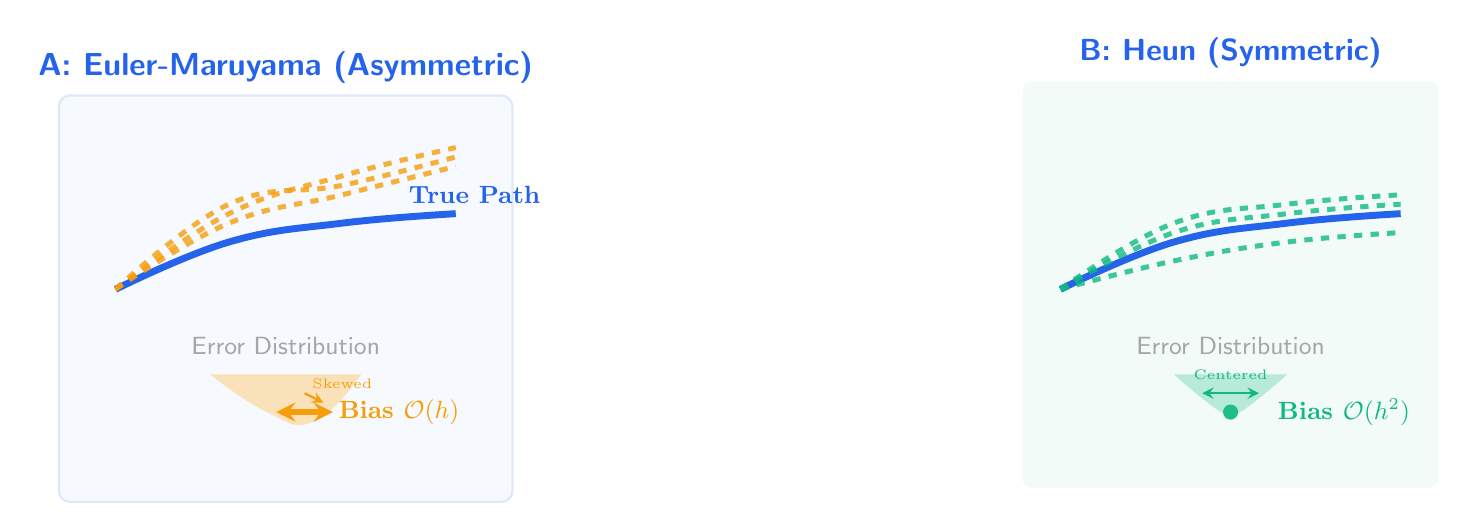
\begin{tikzpicture}[scale=1.2, >=stealth, font=\sffamily]

    % --- Panel A: Euler-Maruyama (Asymmetric Error) ---
    \begin{scope}[shift={(-5,0)}]
        \node[distillBlue, font=\sffamily\bfseries, scale=1.15] at (0, 2.65) {\textbf{A: Euler-Maruyama (Asymmetric)}};
        
        % Background panel with refined styling
        \fill[distillBlue!4, rounded corners=4pt, draw=distillBlue!15, line width=0.8pt] 
            (-2.4,-1.95) rectangle (2.4,2.35);
        
        % True trajectory (conceptual)
        \draw[thick, distillBlue, line width=2.5pt] plot[smooth, tension=0.7] coordinates {(-1.8, 0.3) (-0.6, 0.8) (0.6, 1.0) (1.8, 1.1)};
        \node[distillBlue, font=\small\bfseries] at (2.0, 1.3) {True Path};
        
        % EM paths (biased) - multiple sample paths
        \draw[dashed, distillOrange, line width=1.8pt, opacity=0.8] plot[smooth, tension=0.7] coordinates {(-1.8, 0.3) (-0.6, 1.1) (0.6, 1.5) (1.8, 1.8)};
        \draw[dashed, distillOrange, line width=1.8pt, opacity=0.8] plot[smooth, tension=0.7] coordinates {(-1.8, 0.3) (-0.6, 1.0) (0.6, 1.3) (1.8, 1.6)};
        \draw[dashed, distillOrange, line width=1.8pt, opacity=0.8] plot[smooth, tension=0.7] coordinates {(-1.8, 0.3) (-0.6, 1.2) (0.6, 1.4) (1.8, 1.7)};
        
        % Error distribution visualization
        \node[font=\small\sffamily, color=gray!70] at (0, -0.3) {Error Distribution};
        \fill[distillOrange!40, opacity=0.7] plot[smooth, tension=0.8] coordinates {(-0.8, -0.6) (-0.2, -1.0) (0.3, -1.1) (0.8, -0.6)} -- cycle;
        \draw[thick, distillOrange, <->, line width=2pt] (-0.1, -1.0) -- (0.5, -1.0);
        \node[distillOrange, font=\small\bfseries] at (1.2, -1.0) {Bias $\mathcal{O}(h)$};
        
        % Asymmetry indicator
        \draw[distillOrange, thick, ->] (0.2, -0.8) -- (0.4, -0.9);
        \node[distillOrange, font=\tiny] at (0.6, -0.7) {Skewed};
    \end{scope}

    % --- Panel B: Itô-Heun (Symmetric Error) ---
    \begin{scope}[shift={(5,0)}]
        \node[distillBlue, font=\sffamily\bfseries, scale=1.1] at (0, 2.8) {\textbf{B: Heun (Symmetric)}};
        
        % Background panel
        \fill[distillGreen!5, rounded corners=3pt] (-2.2,-1.8) rectangle (2.2,2.5);
        
        % True trajectory
        \draw[thick, distillBlue, line width=2.5pt] plot[smooth, tension=0.7] coordinates {(-1.8, 0.3) (-0.6, 0.8) (0.6, 1.0) (1.8, 1.1)};
        
        % Heun paths (centered) - multiple sample paths showing symmetry
        \draw[dashed, distillGreen, line width=1.8pt, opacity=0.8] plot[smooth, tension=0.7] coordinates {(-1.8, 0.3) (-0.6, 1.0) (0.6, 1.2) (1.8, 1.3)};
        \draw[dashed, distillGreen, line width=1.8pt, opacity=0.8] plot[smooth, tension=0.7] coordinates {(-1.8, 0.3) (-0.6, 0.6) (0.6, 0.8) (1.8, 0.9)};
        \draw[dashed, distillGreen, line width=1.8pt, opacity=0.8] plot[smooth, tension=0.7] coordinates {(-1.8, 0.3) (-0.6, 0.9) (0.6, 1.1) (1.8, 1.2)};
        
        % Error distribution visualization
        \node[font=\small\sffamily, color=gray!70] at (0, -0.3) {Error Distribution};
        \fill[distillGreen!40, opacity=0.7] plot[smooth, tension=0.8] coordinates {(-0.6, -0.6) (-0.1, -1.0) (0.1, -1.0) (0.6, -0.6)} -- cycle;
        \fill[distillGreen, opacity=0.9] (0, -1.0) circle (0.08);
        \node[distillGreen, font=\small\bfseries] at (1.2, -1.0) {Bias $\mathcal{O}(h^2)$};
        
        % Symmetry indicator
        \draw[distillGreen, thick, <->] (-0.3, -0.8) -- (0.3, -0.8);
        \node[distillGreen, font=\tiny] at (0, -0.6) {Centered};
    \end{scope}

\end{tikzpicture}
\captionsetup{hypcap=false}
{\sloppy\captionof{figure}{\textbf{The Physics of Self-Consistency Bias.} (A) EM's asymmetric error correlates with the training gradient, inducing bias.\\ (B) Symmetric schemes (Itô--Heun) center the error, canceling the leading bias term.}\label{fig:Bias_Physics_R3}\par}
\end{figure}

\subparagraph{2.2. The Itô--Heun (Trapezoidal) Mandate.}
We mandate the \textbf{Itô--Heun (Trapezoidal)} scheme. It achieves the necessary symmetry efficiently, avoiding the costly Stratonovich conversion.

\begin{tcolorbox}[colback=red!10!white, colframe=red!75!black, title={HPC Mandate: Float64 Precision}]
The Heun scheme involves subtracting nearly equal numbers. To prevent catastrophic cancellation, \textbf{64-bit precision (float64)} is mandatory.
\end{tcolorbox}

\paragraph{Pillar 3: Computational Efficiency: QMC and the Geometry of AD.}

\subparagraph{3.1. Data Efficiency: Randomized Quasi-Monte Carlo (rQMC).}
Standard Monte Carlo (MC) converges slowly ($\mathcal{O}(N^{-1/2})$). We mandate rQMC (e.g., scrambled Sobol sequences) for data generation, accelerating convergence towards $\mathcal{O}(N^{-1})$ (Figure \ref{fig:QMC_Convergence_R3}).

\begin{figure}[ht]
\centering
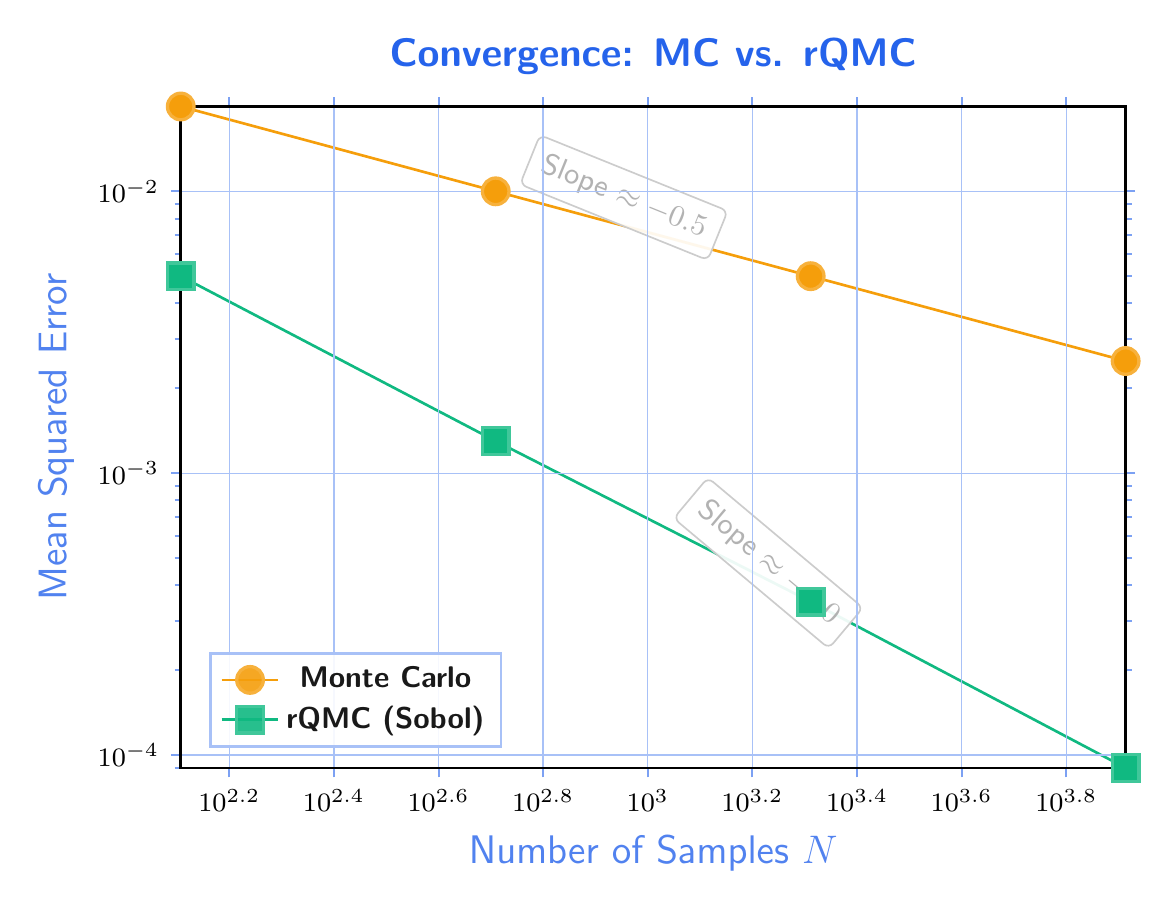
\begin{tikzpicture}[scale=1.2]
    \begin{loglogaxis}[
        title={\large\sffamily\bfseries Convergence: MC vs. rQMC},
        xlabel={\large\sffamily Number of Samples $N$},
        ylabel={\large\sffamily Mean Squared Error},
        legend pos=south west,
        grid=major,
        grid style={thin, distillBlue!20},
        major grid style={distillBlue!40},
        axis lines=box,
        tick style={distillBlue!60},
        title style={font=\sffamily\bfseries, color=distillBlue},
        label style={font=\sffamily, color=distillBlue!80},
        legend style={font=\small\sffamily, fill=white, fill opacity=0.9, draw=distillBlue!40},
        every axis plot/.append style={line width=2pt},
        width=10cm,
        height=7cm,
    ]
    % MC (Slope -0.5) - Enhanced with better markers
    \addplot[
        color=distillOrange, 
        mark=*, 
        mark size=4pt, 
        thick, 
        mark options={fill=distillOrange, draw=distillOrange!80, line width=1pt}
    ] coordinates {
        (128, 0.02) (512, 0.01) (2048, 0.005) (8192, 0.0025)
    };
    \addlegendentry{\sffamily\bfseries Monte Carlo}
    % rQMC (Slope approx -1.0) - Enhanced with better markers
    \addplot[
        color=distillGreen, 
        mark=square*, 
        mark size=4pt, 
        thick, 
        mark options={fill=distillGreen, draw=distillGreen!80, line width=1pt}
    ] coordinates {
        (128, 0.005) (512, 0.0013) (2048, 0.00035) (8192, 0.00009)
    };
    \addlegendentry{\sffamily\bfseries rQMC (Sobol)}
    % Enhanced slope annotations with improved positioning and styling
    \node[
        gray!65, 
        font=\sffamily\small, 
        rotate=-22, 
        align=center,
        fill=white,
        fill opacity=0.92,
        inner sep=4pt,
        rounded corners=2pt,
        draw=gray!40,
        line width=0.5pt
    ] at (axis cs:900, 0.0095) {Slope $\approx -0.5$};
    
    \node[
        gray!65, 
        font=\sffamily\small, 
        rotate=-40, 
        align=center,
        fill=white,
        fill opacity=0.92,
        inner sep=4pt,
        rounded corners=2pt,
        draw=gray!40,
        line width=0.5pt
    ] at (axis cs:1700, 0.00048) {Slope $\approx -1.0$};
    \end{loglogaxis}
\end{tikzpicture}
\captionsetup{hypcap=false}
\captionof{figure}{\textbf{Empirical Convergence Rates.} Randomized Quasi-Monte Carlo (rQMC) demonstrates superior convergence compared to standard Monte Carlo, significantly reducing computational cost for high-dimensional integration.}
    \label{fig:QMC_Convergence_R3}
\end{figure}

\subparagraph{3.2. The Geometry and Efficiency of AD.}
Understanding the cost of Automatic Differentiation (AD) is crucial for efficient implementation of the Malliavin-AD Tower.

\begin{distilldef}{AD Modes and Complexity}
\begin{itemize}
    \item \textbf{Forward Mode (JVP):} Cost scales with input dimension $\mathcal{O}(d_{in})$. Corresponds to the Tangent SDE.
    \item \textbf{Reverse Mode (VJP/Backpropagation):} Cost scales with output dimension $\mathcal{O}(d_{out})$. Corresponds to the Adjoint BSDE.
\end{itemize}
\end{distilldef}

\begin{figure}[ht]
\centering
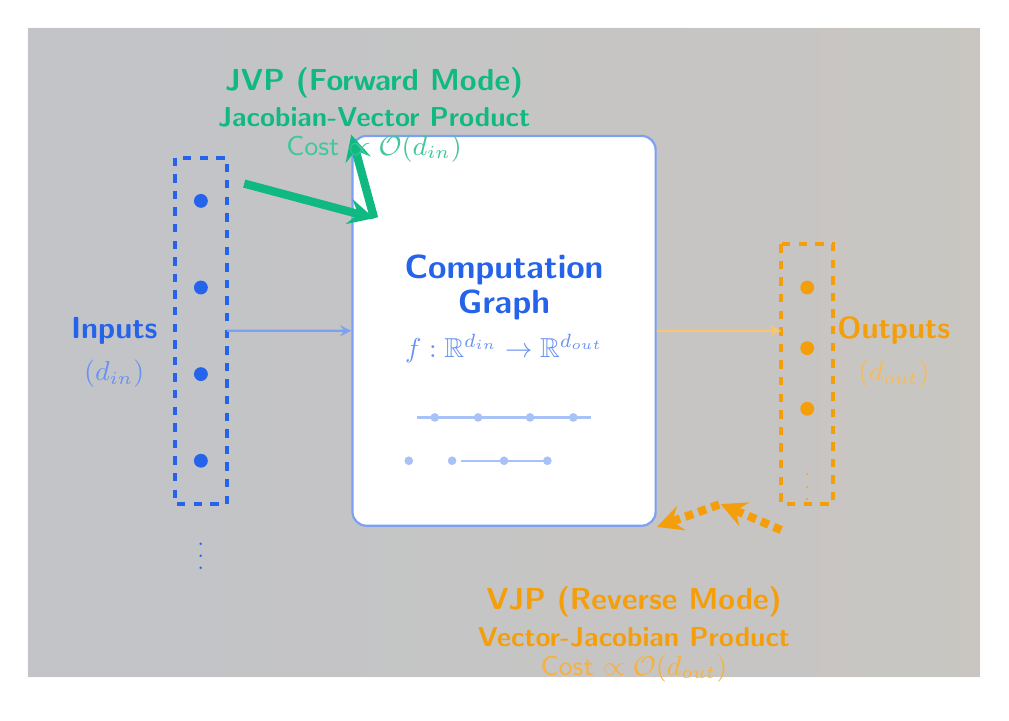
\begin{tikzpicture}[>=stealth, node distance=3cm, scale=1.1, transform shape, font=\sffamily]

    % Background gradient
    \fill[left color=distillBlue!10, right color=distillOrange!10, opacity=0.3] (-2.5,-3.5) rectangle (8.5,4);

    % Input Layer
    \node[distillBlue, font=\sffamily\bfseries] at (-1.5, 0.5) {Inputs};
    \node[distillBlue!70, font=\small] at (-1.5, 0) {$(d_{in})$};
    \draw[distillBlue, thick, dashed, line width=1.5pt] (-0.8, 2.5) rectangle (-0.2, -1.5);
    
    % Input nodes
    \foreach \y in {2, 1, 0, -1} {
    \fill[distillBlue] (-0.5, \y) circle (0.08);
  }
  % Fix font warning: use available font size
  \node[distillBlue, font=\scriptsize] at (-0.5, -2) {$\vdots$};


    % Output Layer
    \node[distillOrange, font=\sffamily\bfseries] at (7.5, 0.5) {Outputs};
    \node[distillOrange!70, font=\small] at (7.5, 0) {$(d_{out})$};
    \draw[distillOrange, thick, dashed, line width=1.5pt] (6.2, 1.5) rectangle (6.8, -1.5);
    
    % Output nodes
    \foreach \y in {1, 0.3, -0.4} {
        \fill[distillOrange] (6.5, \y) circle (0.08);
    }
    \node[distillOrange, font=\tiny] at (6.5, -1.2) {$\vdots$};
    
    % Computation Graph (Enhanced)
    \node (Graph) [draw=distillBlue!60, fill=white, thick, rectangle, rounded corners=5pt, 
                   minimum width=3.5cm, minimum height=4.5cm, 
                   ] 
                   at (3, 0.5) {};
    \node[distillBlue, font=\sffamily\bfseries, scale=1.1] at (3, 1.2) {Computation};
    \node[distillBlue, font=\sffamily\bfseries, scale=1.1] at (3, 0.8) {Graph};
    \node[distillBlue!70, font=\sffamily, scale=0.9] at (3, 0.3) {$f: \mathbb{R}^{d_{in}} \to \mathbb{R}^{d_{out}}$};
    
    % Internal computation representation
    \draw[distillBlue!40, thick] (2, -0.5) -- (4, -0.5);
    \draw[distillBlue!40, thick] (2.5, -1) -- (3.5, -1);
    \foreach \x in {2.2, 2.7, 3.3, 3.8} {
        \fill[distillBlue!40] (\x, -0.5) circle (0.05);
        \fill[distillBlue!40] (\x-0.3, -1) circle (0.05);
    }

    % JVP (Forward Mode) - Enhanced arrow
    \draw[->, line width=3pt, distillGreen] (0, 2.2) -- (1.5, 1.8);
    \draw[->, line width=3pt, distillGreen] (1.5, 1.8) -- (Graph.north west);
    \node[distillGreen, font=\sffamily\bfseries, align=center] at (1.5, 3.2) {
        \textbf{JVP (Forward Mode)}\\
        {\small Jacobian-Vector Product}
    };
    \node[distillGreen!80, font=\small\sffamily] at (1.5, 2.6) {Cost $\propto \mathcal{O}(d_{in})$};

    % VJP (Reverse Mode) - Enhanced arrow
    \draw[<-, line width=3pt, distillOrange, densely dashed] (Graph.south east) -- (5.5, -1.5);
    \draw[<-, line width=3pt, distillOrange, densely dashed] (5.5, -1.5) -- (6.2, -1.8);
    \node[distillOrange, font=\sffamily\bfseries, align=center] at (4.5, -2.8) {
        \textbf{VJP (Reverse Mode)}\\
        {\small Vector-Jacobian Product}
    };
    \node[distillOrange!80, font=\small\sffamily] at (4.5, -3.4) {Cost $\propto \mathcal{O}(d_{out})$};

    % Connection lines (data flow)
    \draw[->, distillBlue!60, thick] (-0.2, 0.5) -- (Graph.west);
    \draw[->, distillOrange!60, thick] (Graph.east) -- (6.2, 0.5);

\end{tikzpicture}
\captionsetup{hypcap=false}
\captionof{figure}{\textbf{The Geometry of Automatic Differentiation.} Forward mode (JVP) scales with input dimension, while reverse mode (VJP) scales with output dimension. This fundamental asymmetry drives the choice of differentiation mode in neural network training.}
\label{fig:AD_Geometry_R3}
\end{figure}

\begin{distillresult}{Efficient Malliavin Implementation}
The Level 1 OSM objective requires gradients of the loss (a scalar, $d_{out}=1$). Therefore, \textbf{Reverse Mode AD (VJP)} is the most efficient method for computing the required Malliavin weights, regardless of the state dimension $d_{in}$.
\end{distillresult}

\paragraph{Pillar 4: The Modern Architecture Stack: Smoothness and Sequences.}

\subparagraph{4.1. The Smoothness Mandate.}
QBSDE solutions are smooth. ReLU networks are inefficient. We mandate smooth activation functions (e.g., SiLU/Swish) and architectures that capture high-frequency components efficiently (e.g., Fourier Feature embeddings \cite{Tancik2020}).

\subparagraph{4.2. The Shift to Sequence Models (Mamba).}
MLPs process time $t$ independently. We pivot to sequence models that process the entire trajectory, capturing long-range dependencies. State Space Models (SSMs), particularly Mamba \cite{GuDao2024_Mamba}, are the 2025 standard, offering linear complexity in sequence length $N$.

\begin{figure}[ht]
\centering
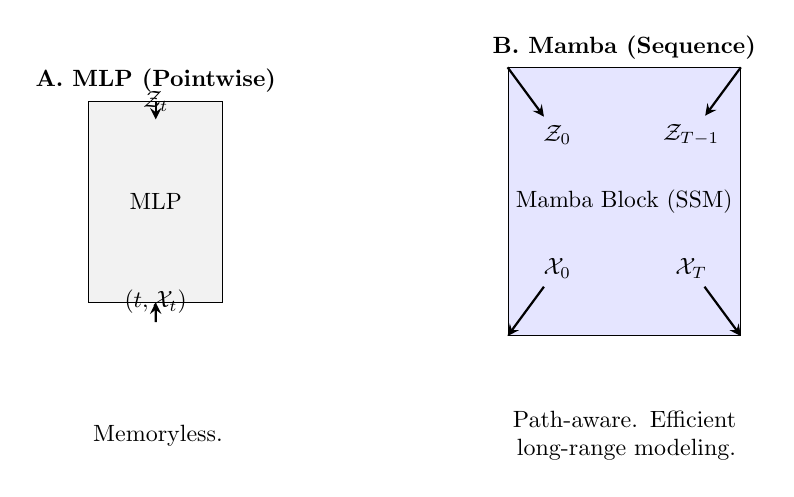
\begin{tikzpicture}[>=stealth, node distance=2cm, scale=0.85, transform shape]

    % === MLP (Pointwise) ===
    \node[draw, rectangle, fill=gray!10, minimum height=3cm, minimum width=2cm, label=above:\textbf{A. MLP (Pointwise)}] (MLP) {MLP};
    \node (Input_t) [below of=MLP, yshift=0.5cm] {$(t, \mathcal{X}_t)$};
    \node (Output_t) [above of=MLP, yshift=-0.5cm] {$\mathcal{Z}_t$};
    \draw[->, thick] (Input_t) -- (MLP);
    \draw[->, thick] (MLP) -- (Output_t);
    \node[text width=3cm, align=center] at (0, -3.5) {Memoryless.};

    % === Sequence Model (Mamba) ===
    \node[draw, rectangle, fill=blue!10, minimum height=4cm, minimum width=3cm, right of=MLP, xshift=5cm, label=above:\textbf{B. Mamba (Sequence)}] (Mamba) {Mamba Block (SSM)};
    
    % Inputs
    \node (X0) [below of=Mamba, xshift=-1cm, yshift=1cm] {$\mathcal{X}_0$};
    \node (XT) [below of=Mamba, xshift=1cm, yshift=1cm] {$\mathcal{X}_T$};
    \draw[->, thick] (X0) -- (Mamba.south west);
    \draw[->, thick] (XT) -- (Mamba.south east);
    
    % Outputs
    \node (Z0) [above of=Mamba, xshift=-1cm, yshift=-1cm] {$\mathcal{Z}_0$};
    \node (ZT) [above of=Mamba, xshift=1cm, yshift=-1cm] {$\mathcal{Z}_{T-1}$};
    \draw[->, thick] (Mamba.north west) -- (Z0);
    \draw[->, thick] (Mamba.north east) -- (ZT);

    \node[text width=4cm, align=center] at (7, -3.5) {Path-aware. Efficient long-range modeling.};

\end{tikzpicture}
\captionsetup{hypcap=false}
\captionof{figure}{\textbf{Architectural Shift.} (A) The traditional pointwise MLP. (B) The modern sequence modeling approach (Mamba) maps the entire state trajectory to the control path.}
    \label{fig:Architecture_Shift_R3}
\end{figure}

% New sophisticated figure showing the complete FBSDE pipeline
\begin{figure}[ht]
\centering
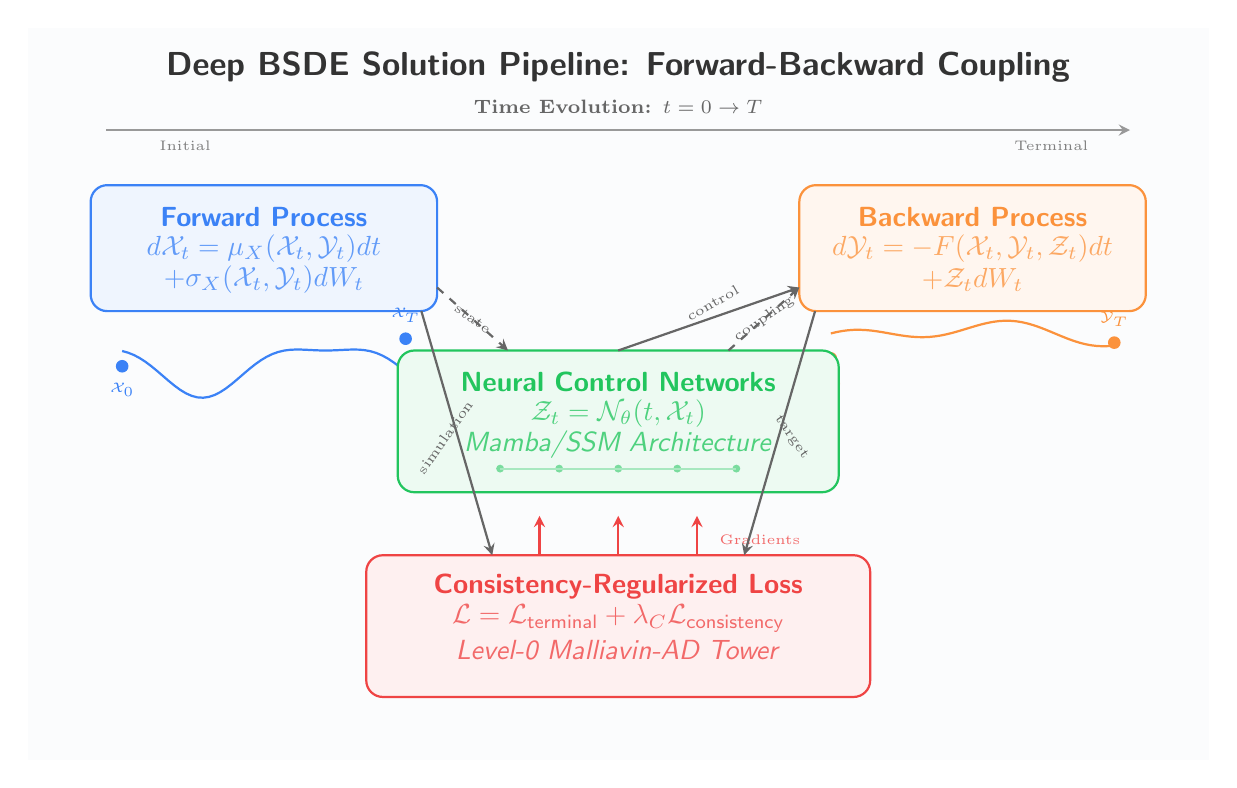
\begin{tikzpicture}[scale=1.0, >=stealth, font=\sffamily\footnotesize, node distance=1.8cm]

    % Define colors with precise matching
    \definecolor{forwardBlue}{RGB}{59, 130, 246}
    \definecolor{backwardOrange}{RGB}{251, 146, 60}
    \definecolor{controlGreen}{RGB}{34, 197, 94}
    \definecolor{lossRed}{RGB}{239, 68, 68}
    \definecolor{bgGray}{RGB}{248, 250, 252}
    
    % Background gradient
    \fill[bgGray, opacity=0.6] (-7.5,-4.5) rectangle (7.5,4.8);
    
    % Title with modern typography
    \node[font=\sffamily\bfseries\large, color=black!80] at (0, 4.3) 
        {\textbf{Deep BSDE Solution Pipeline: Forward-Backward Coupling}};
    
    % === FORWARD PROCESS (Blue) ===
    \begin{scope}[shift={(-4.5, 2)}]
        % Forward process box
        \draw[forwardBlue, thick, rounded corners=6pt, fill=forwardBlue!8] 
            (-2.2, -0.8) rectangle (2.2, 0.8);
        \node[forwardBlue, font=\sffamily\bfseries] at (0, 0.4) {\textbf{Forward Process}};
        \node[forwardBlue!80, font=\sffamily] at (0, 0) {$d\mathcal{X}_t = \mu_X(\mathcal{X}_t, \mathcal{Y}_t) dt$};
        \node[forwardBlue!80, font=\sffamily] at (0, -0.4) {$+ \sigma_X(\mathcal{X}_t, \mathcal{Y}_t) dW_t$};
        
        % State trajectory visualization
        \draw[forwardBlue, thick, samples=50, domain=-1.8:1.8, variable=\x] 
            plot (\x, {-1.5 + 0.3*sin(deg(2*\x)) + 0.1*cos(deg(4*\x))});
        \fill[forwardBlue] (-1.8, -1.5) circle (0.08);
        \fill[forwardBlue] (1.8, -1.15) circle (0.08);
        \node[forwardBlue, font=\tiny] at (-1.8, -1.8) {$\mathcal{X}_0$};
        \node[forwardBlue, font=\tiny] at (1.8, -0.85) {$\mathcal{X}_T$};
    \end{scope}
    
    % === BACKWARD PROCESS (Orange) ===
    \begin{scope}[shift={(4.5, 2)}]
        % Backward process box
        \draw[backwardOrange, thick, rounded corners=6pt, fill=backwardOrange!8] 
            (-2.2, -0.8) rectangle (2.2, 0.8);
        \node[backwardOrange, font=\sffamily\bfseries] at (0, 0.4) {\textbf{Backward Process}};
        \node[backwardOrange!80, font=\sffamily] at (0, 0) {$d\mathcal{Y}_t = -F(\mathcal{X}_t, \mathcal{Y}_t, \mathcal{Z}_t) dt$};
        \node[backwardOrange!80, font=\sffamily] at (0, -0.4) {$+ \mathcal{Z}_t dW_t$};
        
        % Value trajectory visualization (backward)
        \draw[backwardOrange, thick, samples=50, domain=-1.8:1.8, variable=\x] 
            plot (\x, {-1.2 + 0.2*exp(-\x*\x/2) + 0.1*sin(deg(3*\x))});
        \fill[backwardOrange] (1.8, -1.2) circle (0.08);
        \fill[backwardOrange] (-1.8, -1.4) circle (0.08);
        \node[backwardOrange, font=\tiny] at (1.8, -0.9) {$\mathcal{Y}_T$};
        \node[backwardOrange, font=\tiny] at (-1.8, -1.7) {$\mathcal{Y}_0$};
    \end{scope}
    
    % === NEURAL CONTROL NETWORKS (Green) ===
    \begin{scope}[shift={(0, -0.2)}]
        % Control network box
        \draw[controlGreen, thick, rounded corners=6pt, fill=controlGreen!8] 
            (-2.8, -0.9) rectangle (2.8, 0.9);
        \node[controlGreen, font=\sffamily\bfseries] at (0, 0.5) {\textbf{Neural Control Networks}};
        \node[controlGreen!80, font=\sffamily] at (0, 0.1) {$\mathcal{Z}_t = \mathcal{N}_\theta(t, \mathcal{X}_t)$};
        \node[controlGreen!80, font=\sffamily] at (0, -0.3) {\textit{Mamba/SSM Architecture}};
        
        % Network visualization
        \foreach \x in {-1.5, -0.75, 0, 0.75, 1.5} {
            \foreach \y in {-0.6} {
                \fill[controlGreen!60] (\x, \y) circle (0.05);
            }
        }
        \foreach \i in {1,...,4} {
            \draw[controlGreen!40, thick] (-1.5+\i*0.75-0.75, -0.6) -- (-1.5+\i*0.75, -0.6);
        }
    \end{scope}
    
    % === LOSS COMPUTATION (Red) ===
    \begin{scope}[shift={(0, -2.8)}]
        % Loss box
        \draw[lossRed, thick, rounded corners=6pt, fill=lossRed!8] 
            (-3.2, -0.9) rectangle (3.2, 0.9);
        \node[lossRed, font=\sffamily\bfseries] at (0, 0.5) {\textbf{Consistency-Regularized Loss}};
        \node[lossRed!80, font=\sffamily] at (0, 0.1) {$\mathcal{L} = \mathcal{L}_{\text{terminal}} + \lambda_C \mathcal{L}_{\text{consistency}}$};
        \node[lossRed!80, font=\sffamily] at (0, -0.3) {\textit{Level-0 Malliavin-AD Tower}};
        
        % Gradient arrows pointing up
        \foreach \x in {-1, 0, 1} {
            \draw[lossRed, thick, ->] (\x, 0.9) -- (\x, 1.4);
        }
        \node[lossRed!80, font=\tiny] at (1.8, 1.1) {Gradients};
    \end{scope}
    
    % === COUPLING ARROWS ===
    % Forward -> Control (dependency of Z on X)
    \draw[thick, ->, color=black!60, dashed] (-2.3, 1.5) -- (-1.4, 0.7);
    \node[font=\tiny, color=black!60, rotate=-35] at (-1.85, 1.1) {state};
    
    % Control -> Forward (Y dependency in forward drift)
    \draw[thick, ->, color=black!60, dashed] (1.4, 0.7) -- (2.3, 1.5);
    \node[font=\tiny, color=black!60, rotate=35] at (1.85, 1.1) {coupling};
    
    % Control -> Backward (Z in BSDE)
    \draw[thick, ->, color=black!60] (0, 0.7) -- (2.3, 1.5);
    \node[font=\tiny, color=black!60, rotate=30] at (1.2, 1.3) {control};
    
    % Backward -> Loss
    \draw[thick, ->, color=black!60] (2.5, 1.2) -- (1.6, -1.9);
    \node[font=\tiny, color=black!60, rotate=-55] at (2.2, -0.4) {target};
    
    % Forward -> Loss
    \draw[thick, ->, color=black!60] (-2.5, 1.2) -- (-1.6, -1.9);
    \node[font=\tiny, color=black!60, rotate=55] at (-2.2, -0.4) {simulation};
    
    % === TIME FLOW INDICATOR ===
    \draw[thick, ->, color=black!40] (-6.5, 3.5) -- (6.5, 3.5);
    \node[font=\scriptsize\bfseries, color=black!60] at (0, 3.8) {Time Evolution: $t = 0 \to T$};
    \node[font=\tiny, color=black!50] at (-5.5, 3.3) {Initial};
    \node[font=\tiny, color=black!50] at (5.5, 3.3) {Terminal};
    
\end{tikzpicture}
\captionsetup{hypcap=false}
\captionof{figure}{\textbf{Deep BSDE Solution Pipeline.} The forward-backward coupling creates a sophisticated feedback loop: the forward process $\mathcal{X}_t$ (blue) evolves under state-dependent drift and volatility that depend on the backward value $\mathcal{Y}_t$ (orange). Neural networks (green) learn the optimal control $\mathcal{Z}_t$, which appears both in the backward process dynamics and the forward coupling. The consistency-regularized loss (red) trains the entire system end-to-end, with gradients flowing through all components. This architecture breaks the curse of dimensionality by replacing mesh-based PDE solvers with differentiable, path-based simulation.}
\label{fig:Deep_BSDE_Pipeline}
\end{figure}

\paragraph{Pillar 5: Robust Solver Strategy and Optimization.}

\subparagraph{5.1. Handling Coupling: Iterative Decoupling (Picard Iteration).}
The monolithic Deep BSDE approach is unstable for fully coupled systems. We mandate the Picard iteration strategy, transforming the coupled problem into a sequence of stable, decoupled problems.

\begin{distillmethod}{Algorithm: Picard Iteration}
1. Initialize $\Psi^{(0)}$.
2. Iteration $k$: Solve the forward SDE for $\mathcal{X}^{(k)}$ using $\Psi^{(k-1)}$. Then solve the decoupled backward BSDE for $\Psi^{(k)}$ using paths of $\mathcal{X}^{(k)}$.
3. Repeat until convergence.
\end{distillmethod}

\subparagraph{5.2. Robust Optimization and Generalization.}
\begin{itemize}
    \item \textbf{Initialization (Imitate the Expert):} Pre-train the network to match the stationary solution $Y^\infty(X)$. This initializes the optimization in a stable basin.
    \item \textbf{Gradient Clipping by Global Norm:} Essential to prevent gradient explosion.
    \item \textbf{Sharpness-Aware Minimization (SAM):} We use SAM \cite{ForetEtAl2021} to actively seek "flat minima" in the loss landscape, which generalize better to unseen Brownian paths.
\end{itemize}

\paragraph{Pillar 6: Certification, Verification, and UQ.}

\subparagraph{6.1. Implementation Verification: Method of Manufactured Solutions (MMS).}
MMS is the gold standard. We define a known exact solution $u^*$, derive the corresponding manufactured problem $(f^*, g^*)$, and verify the solver converges to $u^*$ at the expected rate ($\mathcal{O}(h^2)$).

\subparagraph{6.2. Solution Certification: A-Posteriori Error Bounds.}
We certify the solution quality using rigorous bounds.

\begin{theorem}[A-Posteriori Error Bound (Bender \& Steiner, 2012; Warin, 2024)]
The error of the learned solution $\hat{\Psi}$ is bounded by the expected integrated residual $\mathcal{R}_t$:
\[
\|\Psi_0 - \hat{\Psi}_0\| \le C \left( \mathbb{E}\left[\int_0^T \|\mathcal{R}_t\|^2 dt\right] \right)^{1/2}.
\]
\end{theorem}
\textbf{Actionable Certification:} The RHS is the consistency loss, providing a rigorous error estimate and stopping criterion.

\subparagraph{6.3. Uncertainty Quantification (UQ): Deep Ensembles.}
We quantify epistemic uncertainty (model uncertainty) using Deep Ensembles (training $M$ independent models) to derive confidence intervals (Figure \ref{fig:UQ_R3}).

\begin{figure}[ht]
\centering
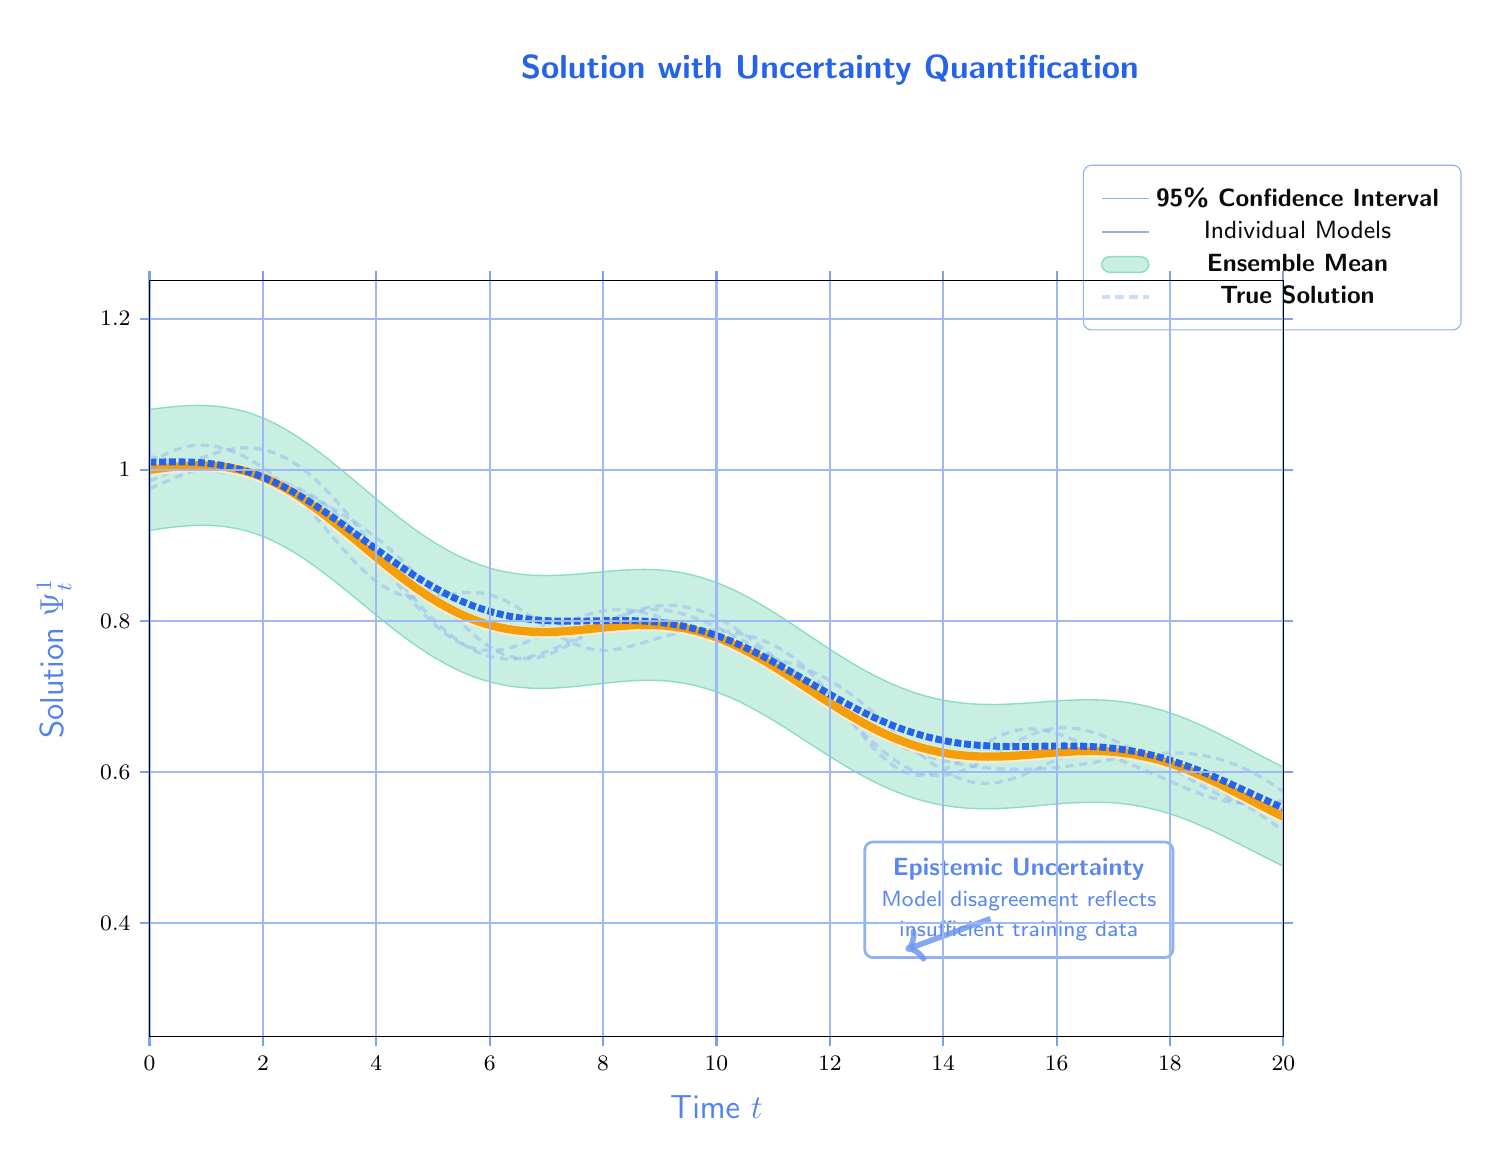
\begin{tikzpicture}[scale=1.2, baseline]
\begin{axis}[
    title={\large\sffamily\bfseries Solution with Uncertainty Quantification},
    xlabel={\large\sffamily Time $t$},
    ylabel={\large\sffamily Solution $\Psi^1_t$},
    xlabel style={font=\large\sffamily, inner sep=8pt},
    ylabel style={font=\large\sffamily, inner sep=8pt},
    title style={font=\large\sffamily\bfseries, color=distillBlue, inner sep=10pt},
    grid=major,
    grid style={thin, distillBlue!25},
    major grid style={distillBlue!45, line width=0.8pt},
    minor grid style={distillBlue!15, line width=0.4pt},
    axis lines=box,
    tick style={distillBlue!60, thick},
    tick label style={font=\sffamily\footnotesize},
    label style={font=\large\sffamily, color=distillBlue!80},
    legend style={
        font=\sffamily\small, 
        fill=white, 
        fill opacity=0.96, 
        draw=distillBlue!50, 
        rounded corners=3pt,
        inner sep=6pt,
        outer sep=3pt
    },
    xmin=0, xmax=20,
    ymin=0.25, ymax=1.25,
    width=12cm, height=8cm,
    legend pos=north east,
    xmajorgrids=true,
    ymajorgrids=true,
]
% Uncertainty band (fill first) - Enhanced with gradient effect
\addplot[name path=upper, draw=none, domain=0:20, samples=120] 
    {exp(-0.03*x + 0.05*sin(deg(x*0.8))) + 0.08*exp(-0.01*x)};
\addplot[name path=lower, draw=none, domain=0:20, samples=120] 
    {exp(-0.03*x + 0.05*sin(deg(x*0.8))) - 0.08*exp(-0.01*x)};
\addplot[fill=distillGreen!30, opacity=0.75, draw=distillGreen!60, line width=0.5pt] 
    fill between[of=upper and lower];
\addlegendentry{\sffamily\bfseries 95\% Confidence Interval}

% Individual ensemble members (showing ensemble diversity) - Enhanced variety
\addplot[color=distillBlue!50, line width=1.2pt, opacity=0.45, densely dashed, samples=100, domain=0:20] 
    {exp(-0.03*x + 0.05*sin(deg(x*0.8))) + 0.032*sin(deg(x*1.3)) + 0.008*cos(deg(x*2.1))};
\addplot[color=distillBlue!50, line width=1.2pt, opacity=0.45, densely dashed, samples=100, domain=0:20] 
    {exp(-0.03*x + 0.05*sin(deg(x*0.8))) - 0.025*cos(deg(x*0.95)) + 0.012*sin(deg(x*1.7))};
\addplot[color=distillBlue!50, line width=1.2pt, opacity=0.45, densely dashed, samples=100, domain=0:20] 
    {exp(-0.03*x + 0.05*sin(deg(x*0.8))) + 0.028*sin(deg(x*0.75)) - 0.015*cos(deg(x*1.1))};
\addplot[color=distillBlue!50, line width=1.2pt, opacity=0.45, densely dashed, samples=100, domain=0:20] 
    {exp(-0.03*x + 0.05*sin(deg(x*0.8))) - 0.021*sin(deg(x*1.4)) + 0.018*cos(deg(x*0.6))};
\addlegendentry{\sffamily Individual Models}

% Mean solution (prominent) - Enhanced with shadow effect
\addplot[color=distillOrange!20, line width=4pt, samples=120, domain=0:20] 
    {exp(-0.03*x + 0.05*sin(deg(x*0.8))) - 0.001};
\addplot[color=distillOrange, line width=3pt, samples=120, domain=0:20] 
    {exp(-0.03*x + 0.05*sin(deg(x*0.8)))};
\addlegendentry{\sffamily\bfseries Ensemble Mean}

% True solution (if known) - Enhanced visibility
\addplot[color=distillBlue, line width=2.5pt, densely dotted, samples=120, domain=0:20] 
    {exp(-0.03*x + 0.04*sin(deg(x*0.8))) + 0.01};
\addlegendentry{\sffamily\bfseries True Solution}
\end{axis}

% Enhanced annotation with professional styling
\node[
    font=\sffamily\small, 
    color=distillBlue!80, 
    align=center,
    fill=white,
    fill opacity=0.95,
    draw=distillBlue!50,
    line width=1pt,
    rounded corners=3pt,
    inner sep=6pt,
    outer sep=2pt
] at (9.2, 1.45) {
    \textbf{Epistemic Uncertainty}\\
    {\footnotesize Model disagreement reflects}\\
    {\footnotesize insufficient training data}
};
\draw[distillBlue!70, ->, line width=2pt, opacity=0.8] (8.9, 1.25) -- (8.0, 0.92);
\end{tikzpicture}
\captionsetup{hypcap=false}
{\sloppy\captionof{figure}{\textbf{Uncertainty Quantification via Deep Ensembles.} The ensemble provides both a robust mean estimate and confidence intervals that quantify epistemic uncertainty.\\ Individual model predictions (dashed lines) show the diversity within the ensemble, while the shaded region represents the 95\% confidence interval derived from ensemble variance.}\label{fig:UQ_R3}\par}
\end{figure}

\paragraph{Pillar 7: The Unified Pipeline}

\begin{tcolorbox}[colback=gray!5!white, colframe=gray!50!black, title={Unified State-of-the-Art Pipeline (2025)}]
\textbf{1. Analytical Preprocessing:}
\begin{itemize}
    \item Apply Cole-Hopf transformation to linearize and remove stiffness.
\end{itemize}
\textbf{2. Architecture and Initialization:}
\begin{itemize}
    \item Architecture: Mamba (SSM) with smooth activations (SiLU) and Fourier Features.
    \item Initialization: "Imitate the Expert" pre-training.
\end{itemize}
\textbf{3. Data Generation and Discretization:}
\begin{itemize}
    \item Sampling: Randomized Quasi-Monte Carlo (rQMC) for $\mathcal{O}(N^{-1})$ convergence.
    \item Integrator: Itô-Heun (Trapezoidal) for $\mathcal{O}(h^2)$ bias reduction.
\end{itemize}
\textbf{4. Solver Strategy and Optimization:}
\begin{itemize}
    \item Solver: Iterative Decoupling (Picard Iteration) for coupled stability.
    \item Optimization: AdamW + SAM for generalization. Gradient Clipping.
    \item Variance Reduction: Malliavin-AD Tower (Level 1 OSM via efficient VJP).
\end{itemize}
\textbf{5. Certification and Reproducibility:}
\begin{itemize}
    \item Verification: Method of Manufactured Solutions (MMS).
    \item Certification: A-Posteriori Error Bounds. UQ via Deep Ensembles.
    \item HPC: Float64 mandatory. JAX implementation. Fixed seeds (20250811).
\end{itemize}
\end{tcolorbox}

\clearpage
\part{Extensions and Outlook}
\label{part:extensions}

\begin{center}
\textit{“The reward for good work is more work.”}
\end{center}

This final part provides a brief survey of several active research frontiers, highlighting current challenges and future opportunities that extend beyond the canonical Markovian, Brownian-driven setting.

\bigskip\hrule\bigskip

\section{Delay and Path-Dependent FBSDEs}
\label{sec:path_dependence}

\paragraph{Motivation.} Many real-world systems exhibit memory. Financial models with transaction costs, macroeconomic models with implementation lags, and reinforcement learning with delayed rewards all lead to dynamics where the coefficients depend on the entire past history of the processes, \(X_{[0,t]}\).

\paragraph{Theory and Numerics.} The analysis of such systems requires the tools of functional Itô calculus. Well-posedness has been established under appropriate Lipschitz conditions on path space \cite{ContFournie2013}. Numerically, this presents a challenge for standard MLP-based deep solvers. Architectures with memory, such as LSTMs, Transformers, or Neural CDEs, are natural candidates for parameterizing the control process \(Z_t\) and have shown promising results.

\section{Jumps and Lévy Processes}
\label{sec:jumps}

\paragraph{Motivation.} Brownian motion is not always sufficient to capture the sudden, discontinuous events seen in finance (market crashes, defaults) or insurance (catastrophic claims). Incorporating jump processes (like Poisson or more general Lévy processes) leads to Partial Integro-Differential Equations (PIDEs) and their probabilistic counterparts, FBSDEs with jumps.

\paragraph{Theory and Numerics.} The BSDE component is augmented with an additional integral with respect to a compensated jump measure. Existence and uniqueness results exist for certain classes of these systems \cite{BarlesBuckdahnPardoux1997}. Numerically, deep learning solvers must be extended to learn the additional jump-related control variable. This involves sampling jump times and sizes during the forward simulation and adds another layer of complexity to the training process. Variance control for the jump component is a key challenge \cite{Bachouch2022}.

\section{Mean-Field Games and FBSDEs}
\label{sec:meanfield}

\paragraph{Motivation.} How does one model a system with a very large number of interacting agents, like a flock of birds, a crowd of pedestrians, or a market with thousands of traders? Mean-field game theory provides a framework by considering the limit as the number of agents goes to infinity. Each agent interacts not with every other agent, but with the statistical distribution (the "mean field") of the entire population.

\paragraph{Theory and Numerics.} The equilibrium in a mean-field game is characterized by a coupled system consisting of a forward HJB equation (for the individual agent's control) and a backward Fokker-Planck equation (for the evolution of the population distribution). This system can be represented as a mean-field FBSDE, where the coefficients depend on the law of the solution \cite{Carmona2016}. Numerically, this is extremely challenging. "Learning-by-particles" methods, where the deep solver is trained on a large ensemble of interacting particles, are the current state-of-the-art. For such systems, architectures that respect permutation symmetry, such as Graph Neural Networks (GNNs), are essential for creating scalable and structurally sound models \cite{MAGNet2019, GMADDPG2023}.

\section{Grand Challenges for 2030}
\label{sec:challenges}

The confluence of probability theory, numerical analysis, and machine learning has opened up exciting new possibilities. Looking ahead, we identify several "grand challenges" that could define the next decade of research in this field:

\begin{enumerate}[label=\textbf{C\arabic*}. ,leftmargin=1.6em]
  \item \textbf{Scaling and Certification:} Solve a 1,000-dimensional, fully coupled FBSDE with a certified error of less than \(10^{-3}\) in under 24 hours of computation. This requires breakthroughs in both algorithmic efficiency (e.g., adaptive sampling, better network architectures) and theoretical understanding (tighter a-posteriori error bounds).
  \item \textbf{Real-Time Control:} Develop pre-trained FBSDE surrogates that can compute optimal hedging strategies (Deltas and Gammas) for complex financial derivatives in real-time. This involves moving from offline training to online inference, potentially using techniques like neural operator learning.
  \item \textbf{Data-Driven Economics:} Solve and calibrate a mean-field game model with \(10^4\) heterogeneous agents to real economic data, providing a new generation of macroeconomic models. This requires tackling the joint challenge of high-dimensional solution and statistical estimation (the "inverse problem"), including issues of non-stationarity and model misspecification.
  \item \textbf{Formal Verification:} Develop methods, possibly leveraging techniques from neural theorem proving, to formally verify that a trained neural network solver respects fundamental theoretical properties like the comparison principle for BSDEs or no-arbitrage constraints in finance. This would be a major step towards building trust in these black-box models for high-stakes applications.
\end{enumerate}

\bigskip\hrule\bigskip

\section*{Epilogue}
\addcontentsline{toc}{section}{Epilogue}

The theory of FBSDEs has journeyed from an abstract mathematical curiosity to a powerful computational tool in less than a century. The path from Kolmogorov’s diffusions to today’s GPU-accelerated deep solvers illustrates a beautiful interplay between theoretical insight and computational innovation. The next breakthroughs will undoubtedly require even deeper collaboration across disciplines. With open-source benchmarks, certifiable algorithms, and ever-more-powerful hardware, forward-backward stochastic reasoning is poised to become an indispensable part of the modern scientist's and engineer's toolkit.

\bigskip
\begin{flushright}
\emph{— End of Manuscript —}
\end{flushright}


\appendix
\part*{Appendices}
\addcontentsline{toc}{part}{Appendices}
\begin{center}
\emph{“The details are not the details. They make the design.”}\\
— Charles Eames
\end{center}
\bigskip

The appendices collect the technical material, proofs, and code snippets that support the main narrative. They are designed to be comprehensive, allowing the dedicated reader to reproduce every result presented in this monograph.

\bigskip
\hrule
\bigskip

\newpage

\section{Proofs and Derivations}
\label{app:proofs}

\subsection{Proof Sketch for the Ma-Yong Theorem \ref{thm:YongMa}}
\label{app:YongMaProof_appendix}
\begin{leanproofbox}{Proof Sketch: Ma-Yong Theorem \ref{thm:YongMa}}
The proof establishes existence and uniqueness for the fully coupled FBSDE \eqref{eq:FBSDE_canonical} under the monotonicity condition \ref{H3}.

\begin{enumerate}
    \item \textbf{Define the Mapping:} Construct a map \(\Phi\) on the space of solutions \(\mathcal{S}^2 \times \mathcal{H}^2\). Given a pair of processes \((\bar{Y}, \bar{Z})\), \(\Phi\) produces a new pair \((Y,Z)\) as follows:
    \begin{enumerate}
        \item Solve the forward SDE for \(X\) using \((\bar{Y}, \bar{Z})\) in the coefficients:
        \[ dX_t = \bm\mu(t, X_t, \bar{Y}_t, \bar{Z}_t)dt + \bm\sigma(t, X_t, \bar{Y}_t)dW_t. \]
        Under \ref{H1}-\ref{H2}, this SDE has a unique solution.
        \item With this path \(X\), solve the backward SDE for \((Y,Z)\):
        \[ dY_t = -f(t, X_t, Y_t, Z_t)dt + Z_t dW_t, \quad Y_T = g(X_T). \]
        This is a standard BSDE which has a unique solution under \ref{H1}-\ref{H2}.
    \end{enumerate}
    A solution to the original FBSDE is a fixed point of this map, i.e., \(\Phi(Y,Z) = (Y,Z)\).

    \item \textbf{Show Contraction:} The core of the proof is to show that \(\Phi\) is a contraction mapping on a suitable space. This is where the monotonicity condition \ref{H3} is essential. Consider two inputs \((\bar{Y}^1, \bar{Z}^1)\) and \((\bar{Y}^2, \bar{Z}^2)\) and their corresponding outputs \((Y^1, Z^1)\) and \((Y^2, Z^2)\). Let \(\delta Y = Y^1 - Y^2\), etc. Applying Itô's formula to \(e^{\beta t}\|\delta Y_t\|^2\) for a well-chosen \(\beta > 0\) and using the monotonicity condition \ref{H3} leads to an inequality of the form:
    \[ \mathbb{E}[e^{\beta t}\|\delta Y_t\|^2] + \mathbb{E}\left[\int_t^T e^{\beta s}\|\delta Z_s\|^2 ds\right] \le C \mathbb{E}\left[\int_t^T e^{\beta s} (\|\delta \bar{Y}_s\|^2 + \|\delta \bar{Z}_s\|^2) ds\right]. \]
    For a sufficiently small time horizon \(T\), or by choosing \(\beta\) large enough, the map \(\Phi\) becomes a contraction on the weighted space.

    \item \textbf{Extend to Global Solution:} The contraction property on a small interval \([T-\delta, T]\) guarantees a unique solution on that interval. This solution can then be "stitched" together backward in time, extending the uniqueness to the full interval \([0,T]\).
\end{enumerate}
The Banach fixed-point theorem then ensures the existence of a unique solution.
\end{leanproofbox}

\subsection{Derivations for the Two-Agent GE Model}
\label{app:WealthShare}
\begin{leanproofbox}{Technical Derivations}
\paragraph{A. Derivation of the Wealth Share SDE (Eq. \ref{eq:wealth_share_SDE_new_main}).}
We derive the SDE for \(X_t = W_{1t}/S_t\). Applying Itô's quotient rule:
\begin{equation*}
\frac{dX_t}{X_t} = \frac{dW_{1t}}{W_{1t}} - \frac{dS_t}{S_t} - \text{Cov}_t\left(\frac{dW_{1t}}{W_{1t}}, \frac{dS_t}{S_t}\right) + \text{Var}_t\left(\frac{dS_t}{S_t}\right).
\end{equation*}
The diffusion term is \(\sigma_X/X_t = \sigma_{W_1} - \sigma_S\). Using the optimal portfolios \(\pi_{it}^* = \kappa_t/(\gamma_i \sigma_{St})\), we have \(\sigma_{W_i} = \pi_{it}^*\sigma_{St} = \kappa_t/\gamma_i\). Market clearing implies \(\sigma_S = X_t \sigma_{W_1} + (1-X_t)\sigma_{W_2}\).
\begin{align*}
\sigma_X &= X_t(\sigma_{W_1} - \sigma_S) = X_t(1-X_t)(\sigma_{W_1}-\sigma_{W_2}) \\
&= X_t(1-X_t)\kappa_t\left(\frac{1}{\gamma_1}-\frac{1}{\gamma_2}\right).
\end{align*}
The drift term involves substituting the drifts of \(W_{1t}\) and \(S_t\), incorporating consumption rates \(c_{it}/W_{it} = 1/Y^i_t\), and the covariance terms. After algebraic simplification, it yields an expression for $\mu_X$.

\paragraph{B. Derivation of the Transformed SDE for \(\mathcal{X}_t\).}
We apply Itô's lemma to \(\mathcal{X}_t = h(X_t) = \log(X_t/(1-X_t))\). The derivatives are \(h'(x) = \frac{1}{x(1-x)}\) and \(h''(x) = -\frac{1-2x}{(x(1-x))^2}\).
\begin{equation*}
d\mathcal{X}_t = h'(X_t) dX_t + \frac{1}{2} h''(X_t) (dX_t)^2.
\end{equation*}
The diffusion term is \(\sigma_{\mathcal{X}} = h'(X_t)\sigma_X(t) = \frac{1}{X_t(1-X_t)} \sigma_X(t)\), which simplifies to $\kappa_t(\frac{1}{\gamma_1}-\frac{1}{\gamma_2})$.
The drift term is \(\mu_{\mathcal{X}} = h'(X_t)\mu_X(t) + \frac{1}{2} h''(X_t)\sigma_X(t)^2$. Substituting the expressions for \(\mu_X\) and \(\sigma_X\) and simplifying yields the final drift for $\mathcal{X}_t$.
\end{leanproofbox}

\section{Benchmark Problem Specifications}
\label{app:benchmark_details}

This appendix provides the explicit coefficient functions for the benchmark problems introduced in Part \ref{part:benchmarks}.

\subsection{B.1: Allen-Cahn Equation}
The FBSDE system is \(dX_t = dW_t\) and \(dY_t = -f(Y_t)dt + Z_t dW_t\).
\begin{itemize}
    \item \textbf{Forward drift} \(\bm\mu(t,x,y,z) = 0\).
    \item \textbf{Forward volatility} \(\bm\sigma(t,x,y) = I_d\) (identity matrix).
    \item \textbf{BSDE driver} \(f(t,x,y,z) = y - y^3\).
    \item \textbf{Terminal condition} A common choice is \(g(x) = \frac{1}{1+\exp(x_1)}\) or another sigmoid-like function to initialize the phase separation.
\end{itemize}

\subsection{B.2: HJB Equation (LQ Control)}
Consider controlling \(dX_t = \alpha_t dt + \sqrt{2}dW_t\) to minimize \(\mathbb{E}[\int_0^T (\alpha_t^2 + \|X_t\|^2) dt + \|X_T\|^2]\). The value function \(u(t,x)\) solves \(\partial_t u + \Delta u - \frac{1}{2} \|\nabla u\|^2 + \frac{1}{2}\|x\|^2 = 0\).
\begin{itemize}
    \item \textbf{Forward SDE:} The optimal control is \(\alpha_t^* = -\nabla u(t,X_t)\). The PDE solution is \(u(t,x) = \coth(T-t+c)\|x\|^2/2 + \dots\), so \(\nabla u = \coth(T-t+c)x\). This gives a coupled system.
    \item \textbf{BSDE driver} \(f(t,x,y,z) = -\frac{1}{2}\|z\|^2 + \frac{1}{2}\|x\|^2\).
    \item \textbf{Terminal condition} \(g(x) = \|x\|^2\).
\end{itemize}

\subsection{B.3: Nonlinear Black-Scholes}
The FBSDE system is \(dX_t = rX_t dt + \sigma X_t dW_t\) and \(dY_t = -f(Y_t, Z_t)dt + Z_t dW_t\).
\begin{itemize}
    \item \textbf{Forward drift} \(\mu(t,x) = rx\).
    \item \textbf{Forward volatility} \(\sigma(t,x) = \sigma x\).
    \item \textbf{BSDE driver} \(f(t,x,y,z) = -ry + R(y - z/\sigma)\), where \(R\) is a nonlinear function, e.g., \(R(q) = \delta |q|\).
    \item \textbf{Terminal condition} \(g(x) = (x-K)^+\) for a European call option.
\end{itemize}

\section{Computational Appendix: The Two-Agent GE Model Implementation}
\label{app:GE_impl}
\addcontentsline{toc}{section}{Appendix C: GE Model Implementation}

This appendix provides a detailed, pedagogical walkthrough of the complete JAX implementation for solving the two-agent general equilibrium model. The goal is to guide a graduate student through each component, explaining not just the "what" but the "why" of the code structure and numerical choices. We implement the numerically stabilized system using the Logit/Log transformations (Section \ref{subsec:GE_transforms}) and the Deep BSDE method with a Heun integrator and a consistency-regularized loss, paying special attention to the QBSDE structure.

\subsection{C.1: Preamble and Reproducibility Audit}
Before defining the model, we perform a reproducibility audit. This ensures that any user running this code is aware of the exact software environment and configurations, which is critical for numerical work. We mandate 64-bit precision for accuracy, especially given the sensitivity of the QBSDE dynamics and the small correction terms in the Heun integrator.

\begin{lstlisting}[language=Python, caption={C.1: Reproducibility and Precision Audit.}, label={lst:audit_app_appendix}]
import jax
import jax.numpy as jnp
import jax.random as jr
from typing import Tuple
import equinox as eqx
import optax

# --- C.1.1: Mandate float64 for precision ---
# The Heun scheme's corrector step and QBSDE dynamics involve small differences,
# making 64-bit precision essential for numerical stability and accuracy.
jax.config.update("jax_enable_x64", True)

# --- C.1.2: Log environment for reproducibility ---
# JAX's default PRNG changed after version 0.4.25. We rely on the modern 'threefry'
# implementation and fixed seeds for reproducibility.
print("--- COMPUTATIONAL ENVIRONMENT AUDIT ---")
print(f"JAX version: {jax.__version__}")
print(f"X64 enabled: {jax.config.jax_enable_x64}")
print(f"Default PRNG implementation: {jax.config.jax_default_prng_impl}")
print("------------------------------------")
\end{lstlisting}

\subsection{C.2: Defining the Transformed Economic Model}
Our first step is to encapsulate all the economic logic into a single, well-defined class. We use an `equinox.Module`, which behaves like a Python dataclass but is compatible with JAX's functional programming paradigm (JIT compilation, automatic differentiation, etc.). This class will hold all model parameters and implement the functions for the transformed FBSDE system.

\begin{lstlisting}[language=Python, caption={C.2: Transformed Lucas Model FBSDE Coefficients in JAX.}, label={lst:lucas_jax_transformed_app_appendix}]
class LucasGEModel(eqx.Module):
    """
    Defines the primitives and transformed FBSDE system for the GE model.
    This module holds all parameters and implements the core economic functions.
    """
    # --- Economic Primitives ---
    # `eqx.static_field` tells Equinox that these fields are compile-time 
    # constants, not trainable parameters. This is crucial for efficient JIT compilation.
    mu_D: float = eqx.static_field()
    sigma_D: float = eqx.static_field()
    T: float = eqx.static_field()
    N: int = eqx.static_field()
    
    # Agent-specific parameters. These are fixed but not marked static, as one
    # might want to perform inference on them in other contexts.
    rho: jnp.ndarray  # Shape (2,) for two agents' discount rates
    gamma: jnp.ndarray # Shape (2,) for risk aversions

    # --- Derived Numerical Constants ---
    @property
    def h(self): 
        """Time step size."""
        return self.T / self.N
    @property
    def sqrt_h(self): 
        """Square root of time step size, for scaling Brownian increments."""
        return jnp.sqrt(self.h)

    def _get_equilibrium(self, cal_X, cal_Y):
        """
        Computes key equilibrium quantities from transformed state variables.
        cal_X: logit(X), cal_Y: log(Y)
        """
        # 1. Inverse transform state variables to their economic meaning
        X = jax.nn.sigmoid(cal_X) # logit^{-1} -> wealth share in (0,1)
        
        # 2. Compute consumption shares (lambda_c)
        # CRITICAL: Implemented using log-space arithmetic for numerical stability,
        # especially when X is close to 0 or 1. The naive formula:
        # lambda_c1 = (X/exp(cal_Y1)) / (X/exp(cal_Y1) + (1-X)/exp(cal_Y2))
        # is prone to underflow/overflow.
        log_c1_numerator = jnp.log(X) - cal_Y[..., 0]
        log_c2_numerator = jnp.log(1.0 - X) - cal_Y[..., 1]
        # jax.nn.logaddexp(a,b) is a stable way to compute log(exp(a)+exp(b))
        log_denominator = jnp.logaddexp(log_c1_numerator, log_c2_numerator)
        
        lambda_c1 = jnp.exp(log_c1_numerator - log_denominator)
        lambda_c2 = 1.0 - lambda_c1
        
        # 3. Compute aggregate risk aversion and prices, as per theory
        inv_Gamma = (lambda_c1 / self.gamma[0]) + (lambda_c2 / self.gamma[1])
        Gamma = 1.0 / inv_Gamma
        kappa = Gamma * self.sigma_D # Market price of risk
        R_agg = lambda_c1 * self.rho[0] + lambda_c2 * self.rho[1] # Agg. discount rate
        # Generalized Ramsey rule for the risk-free rate
        r = R_agg + Gamma * self.mu_D - 0.5 * Gamma * (Gamma + 1.0) * self.sigma_D**2
        return kappa, r, X, lambda_c1, lambda_c2

    def forward_sde(self, t, cal_X, cal_Y):
        """Computes drift (mu_calX) and volatility (sigma_calX) of the transformed forward process."""
        kappa, _, X, _, _ = self._get_equilibrium(cal_X, cal_Y)
        risk_tol_diff = (1.0 / self.gamma[0]) - (1.0 / self.gamma[1])
        
        # Volatility of transformed process cal_X is constant w.r.t. X
        sigma_calX = kappa * risk_tol_diff
        
        # Ito drift for cal_X (logit transform) requires an Ito correction term
        mu_X_untransformed = X * (1.0 - X) * (jnp.exp(-cal_Y[..., 1]) - jnp.exp(-cal_Y[..., 0]))
        ito_correction = -0.5 * (1.0 - 2.0 * X) * sigma_calX**2
        mu_calX = (mu_X_untransformed / (X * (1.0 - X))) + ito_correction
        return mu_calX, sigma_calX

    def driver(self, t, cal_X, cal_Y, cal_Z):
        """Computes the transformed driver F for the backward process cal_Y."""
        kappa, r, _, _, _ = self._get_equilibrium(cal_X, cal_Y)
        # Reshape for broadcasting against agent-specific dimensions
        rho_b = jnp.expand_dims(self.rho, 0)
        gamma_b = jnp.expand_dims(self.gamma, 0)
        r_b = jnp.expand_dims(r, -1)
        kappa_b = jnp.expand_dims(kappa, -1)

        # This is the driver for d(cal_Y) = -F dt + cal_Z dW, derived via Ito's lemma
        # on cal_Y = log(Y). It has the QBSDE structure.
        intertemporal_hedging = ((1.0 - gamma_b) / gamma_b) * (r_b + 0.5 * gamma_b * kappa_b**2)
        ito_term_from_log = 0.5 * cal_Z**2
        F = (1.0 - rho_b - intertemporal_hedging) - (1.0 - gamma_b) * cal_Z * kappa_b + ito_term_from_log
        return F
        
    def terminal_g(self, cal_X):
        """Terminal condition approximation: log(1/rho_i)."""
        # This is the stationary value for a representative agent, used as an
        # approximation for the infinite horizon problem.
        g = -jnp.log(self.rho)
        # Tile to match the batch dimension of cal_X
        return jnp.broadcast_to(g, (cal_X.shape[0], 2))
\end{lstlisting}

\subsection{C.3: Neural Network Architecture (Equinox)}
We define the neural networks that will approximate the unknown functions. `ControlApproximator` learns the function \(Z(t,X)\). In the previous draft, this included a `tanh` saturation for stability. However, following the advanced methodology in Section \ref{subsec:GE_discretization_full_R3}, we now rely on the Cole-Hopf transformation to handle the quadratic term analytically. This simplifies the network architecture, as explicit stabilization is no longer required.

\begin{lstlisting}[language=Python, caption={C.3: Equinox Modules for the Deep BSDE Solver (Post Cole-Hopf).}, label={lst:equinox_mlp_app_appendix}]
class ControlApproximator(eqx.Module):
    """
    Neural network approximating the control Z(t, X) -> R^2.
    After the Cole-Hopf transformation, the BSDE is no longer quadratic,
    so we do not need explicit stabilization like tanh saturation.
    """
    mlp: eqx.nn.MLP
    T_max: float = eqx.static_field()

    def __init__(self, key, T_max):
        self.T_max = T_max
        # Input: 2 features (normalized time, transformed state cal_X)
        # Output: 2 features (cal_Z for agent 1, cal_Z for agent 2)
        self.mlp = eqx.nn.MLP(in_size=2, out_size=2, width_size=128, depth=3, 
                              activation=jax.nn.silu, key=key)

    def __call__(self, t, cal_X):
        # Normalize time to [0,1] as a standard practice for NNs
        t_norm = t / self.T_max
        # Ensure t_norm is broadcast to the same shape as cal_X for stacking
        t_b = jnp.broadcast_to(t_norm, cal_X.shape)
        # Input to MLP should be of shape (batch_size, 2)
        mlp_in = jnp.stack([t_b, cal_X], axis=-1)
        return self.mlp(mlp_in)

class InitialValue(eqx.Module):
    """A simple container for the trainable parameter Y0."""
    calY0: jnp.ndarray
    def __init__(self, guess): self.calY0 = guess
    def __call__(self): return self.calY0
\end{lstlisting}

\subsection{C.4: The Simulation Loop and Loss Function}
This is the heart of the solver. The \texttt{compute\_loss} function performs the forward simulation of the FBSDE system for a batch of paths and calculates the total loss. It is designed to be JIT-compiled for maximum performance. The Heun scheme is correctly applied to both forward and backward processes to reduce bias, and the consistency loss is implemented with a \texttt{stop\_gradient} to prevent the optimization from becoming degenerate.

\begin{lstlisting}[language=Python, caption={C.4: JAX Implementation of the Consistency-Regularized Loss with Heun Scheme.}, label={lst:jax_loss_fn_app_appendix}]
def compute_loss(models: Tuple, batch_calX0: jnp.ndarray, econ_model: LucasGEModel, 
                 key: jr.PRNGKey, lambda_C: float):
    model_calY0, model_Z = models
    h, N, sqrt_h = econ_model.h, econ_model.N, econ_model.sqrt_h
    keys = jr.split(key, N)
    batch_size = batch_calX0.shape[0]
    
    # Vectorize functions to operate over the batch dimension.
    # `jax.vmap` is a key transformation for batching operations on a GPU/TPU.
    vmap_Z = jax.vmap(model_Z, in_axes=(None, 0)) # Map over cal_X, keep t fixed
    vmap_fwd = jax.vmap(econ_model.forward_sde, in_axes=(None, 0, 0))
    vmap_driver = jax.vmap(econ_model.driver, in_axes=(None, 0, 0, 0))

    # `jax.lax.scan` is a functional loop, essential for JIT-compiling simulations.
    # It iterates over a sequence (time steps), carrying a state (X_k, Y_k).
    def heun_step(carry, step_data):
        calX_k, calY_k = carry
        k, key_step = step_data
        t_k = k * h
        dW = jr.normal(key_step, (batch_size, 1)) * sqrt_h
        
        # --- Predictor values (evaluated at time k) ---
        calZ_k = vmap_Z(t_k, calX_k)
        mu_X_k, sigma_X_k = vmap_fwd(t_k, calX_k, calY_k)
        F_k = vmap_driver(t_k, calX_k, calY_k, calZ_k)
        
        # --- Predictor step for X and Y ---
        calX_pred = calX_k + mu_X_k * h + sigma_X_k * dW[:, 0]
        calY_pred = calY_k - F_k * h + calZ_k * dW
        
        # --- Corrector values (evaluated at time k+1 using predicted values) ---
        calZ_pred = vmap_Z(t_k + h, calX_pred)
        mu_X_pred, _ = vmap_fwd(t_k + h, calX_pred, calY_pred)
        F_pred = vmap_driver(t_k + h, calX_pred, calY_pred, calZ_pred)
        
        # --- Heun Update for X and Y ---
        calX_kp1 = calX_k + 0.5 * (mu_X_k + mu_X_pred) * h + sigma_X_k * dW[:, 0]
        calY_kp1 = calY_k - 0.5 * (F_k + F_pred) * h + 0.5 * (calZ_k + calZ_pred) * dW
        
        # --- Loss Calculation ---
        # Calculate the one-step residual for the consistency loss.
        # We use stop_gradient on the target to prevent the loss from being zero by construction.
        target_Y_kp1 = jax.lax.stop_gradient(calY_k - 0.5 * (F_k + F_pred) * h + 0.5 * (calZ_k + calZ_pred) * dW)
        residual = calY_kp1 - target_Y_kp1
        
        return (calX_kp1, calY_kp1), jnp.sum(residual**2, axis=-1)

    calY0_batch = jnp.broadcast_to(model_calY0(), (batch_size, 2))
    init_carry = (batch_calX0, calY0_batch)
    
    (calX_N, calY_N), residuals_sq_hist = jax.lax.scan(
        heun_step, init_carry, (jnp.arange(N), keys)
    )
    
    # --- Total Loss Computation ---
    # L_T: Terminal Loss (standard Deep BSDE loss)
    g_XN = econ_model.terminal_g(calX_N)
    terminal_loss = jnp.mean(jnp.sum((calY_N - g_XN)**2, axis=-1))
    
    # L_C: Consistency Loss (Level 0 of Malliavin-AD Tower)
    consistency_loss = jnp.mean(residuals_sq_hist)

    total_loss = terminal_loss + lambda_C * consistency_loss
    return total_loss, {"L_T": terminal_loss, "L_C": consistency_loss}

# Define the function that computes loss and gradients.
# This is done once at the top level for efficiency.
# `has_aux=True` tells JAX that our loss function returns auxiliary data (the dict).
loss_and_grad_fn = eqx.filter_value_and_grad(compute_loss, has_aux=True)
\end{lstlisting}

\subsection{C.5: Training Setup and Acceptance Tests}
The main training loop uses Optax for optimization and calls the JIT-compiled \texttt{make\_step}. After training, it runs a suite of acceptance tests to verify the economic and numerical consistency of the learned solution. These tests are crucial for building confidence in the results and correspond directly to the theoretical properties discussed in the main text.

\begin{lstlisting}[language=Python, caption={C.5: Training Loop, JIT-compiled Step, and Acceptance Tests.}, label={lst:jax_training_app_appendix}]
@eqx.filter_jit
def make_step(models, opt_state, key, econ_model, batch_size, lambda_C, optimizer):
    """Performs one step of optimization. JIT-compiled for efficiency."""
    # We start from a fixed initial state for simplicity (logit(0.5) = 0).
    batch_calX0 = jnp.zeros((batch_size,))
    
    # Compute loss and gradients by calling the pre-defined function.
    (loss, aux), grads = loss_and_grad_fn(models, batch_calX0, econ_model, key, lambda_C)
    
    # Update parameters using the optimizer.
    updates, opt_state = optimizer.update(grads, opt_state, models)
    models = eqx.apply_updates(models, updates)
    return models, opt_state, loss, aux

def run_acceptance_tests(trained_models, econ_model):
    """Runs a suite of tests to verify the solution."""
    print("\n--- RUNNING ACCEPTANCE TESTS ON FINAL MODEL ---")
    model_calY0, model_Z = trained_models
    
    # T1: Market Clearing Test
    print("T1: Verifying market clearing for consumption...")
    calY0 = model_calY0()
    test_calX = jnp.array([-10.0, -1.0, 0.0, 1.0, 10.0])
    vmap_eq = jax.vmap(econ_model._get_equilibrium, in_axes=(0, 0))
    calY_tiled = jnp.broadcast_to(calY0, (test_calX.shape[0], 2))
    _, _, _, lambda_c1, lambda_c2 = vmap_eq(test_calX, calY_tiled)
    total_share = lambda_c1 + lambda_c2
    assert jnp.allclose(total_share, 1.0, atol=1e-12), "T1 Failed: Market clearing!"
    print("✅ T1 Passed: Market Clearing holds.")

    # T2: Boundary Safety Test
    print("T2: Verifying boundary safety...")
    key_test = jr.PRNGKey(42)
    test_batch_size = 10000
    test_calX0 = jnp.zeros((test_batch_size,))
    init_carry = (test_calX0, jnp.broadcast_to(calY0, (test_batch_size, 2)))
    
    vmap_fwd_test = jax.vmap(econ_model.forward_sde, in_axes=(None, 0, 0))

    def test_sim_step(carry, step_data):
        calX_k, calY_k = carry
        t_k = step_data * econ_model.h
        dW = jr.normal(jr.PRNGKey(step_data), (test_batch_size, 1)) * econ_model.sqrt_h
        mu_X_k, sigma_X_k = vmap_fwd_test(t_k, calX_k, calY_k)
        calX_kp1 = calX_k + mu_X_k * econ_model.h + sigma_X_k * dW[:,0]
        return (calX_kp1, calY_k), calX_kp1

    _, X_hist = jax.lax.scan(test_sim_step, init_carry, jnp.arange(econ_model.N))
    
    X_untransformed = jax.nn.sigmoid(X_hist)
    assert jnp.all(X_untransformed > 1e-15) and jnp.all(X_untransformed < 1.0 - 1e-15), "T2 Failed: Boundary hit!"
    print("✅ T2 Passed: Boundaries are inaccessible.")
    print("---------------------------------------------")

# --- Main Execution Block ---
if __name__ == '__main__':
    key = jr.PRNGKey(20250811)
    key_model, key_train = jr.split(key)
    
    params = {'mu_D': 0.02, 'sigma_D': 0.2, 'rho': jnp.array([0.03, 0.04]), 
              'gamma': jnp.array([2.0, 5.0]), 'T': 30.0, 'N': 100}
    econ_model = LucasGEModel(**params)
    
    model_Z = ControlApproximator(key_model, econ_model.T)
    model_calY0 = InitialValue(-jnp.log(econ_model.rho))
    models = (model_calY0, model_Z)
    
    optimizer = optax.adamw(learning_rate=1e-3)
    opt_state = optimizer.init(eqx.filter(models, eqx.is_array))

    print("\nStarting JAX/Equinox training with Heun integrator and consistency loss...")
    for step in range(5001):
        key_train, key_batch = jr.split(key_train)
        models, opt_state, loss, aux = make_step(
            models, opt_state, key_batch, econ_model, 2048, lambda_C=0.5, optimizer=optimizer
        )
        if step % 1000 == 0:
            final_Y0_module, _ = models
            Y0_untransformed = jnp.exp(final_Y0_module.calY0)
            print(f"Step {step:4d} | Loss: {loss:.5f} | L_T: {aux['L_T']:.5f} | L_C: {aux['L_C']:.5f} "
                  f"| Y0_1: {Y0_untransformed[0]:.4f}, Y0_2: {Y0_untransformed[1]:.4f}")

    run_acceptance_tests(models, econ_model)
\end{lstlisting}

\newpage
\begin{filecontents*}{\jobname.bib}
@incollection{Bachouch2022,
  title={Deep learning for pricing and hedging of derivatives on assets with jumps},
  author={Bachouch, A. and Hur{\'e}, C. and Langren{\'e}, N. and Pham, H.},
  booktitle={Machine Learning and Data Sciences for Financial Markets},
  pages={209--246},
  year={2022},
  publisher={Chapman and Hall/CRC}
}
@article{BarlesBuckdahnPardoux1997,
  title={Backward stochastic differential equations and integral-partial differential equations},
  author={Barles, G. and Buckdahn, R. and Pardoux, E.},
  journal={Stochastics and Stochastics Reports},
  volume={60},
  number={1-2},
  pages={57--83},
  year={1997}
}
@article{Beck2019,
    title={Deep splitting method for parabolic {PDEs}},
    author={Beck, Christian and Becker, Sebastian and Cheridito, Patrick and Jentzen, Arnulf and Neufeld, Ariel},
    journal={arXiv preprint arXiv:1907.03452},
    year={2019}
}
@article{BenderSteiner2012,
  title={A Posteriori Estimates for Backward SDEs},
  author={Bender, C. and Steiner, J.},
  journal={SIAM/ASA Journal on Uncertainty Quantification},
  volume={1},
  number={1},
  pages={139--163},
  year={2012}
}
@article{Carmona2016,
  title={Mean field games with common noise},
  author={Carmona, R. and Delarue, F. and Lacker, D.},
  journal={The Annals of Probability},
  volume={44},
  number={6},
  pages={3740--3803},
  year={2016}
}
@article{ChanKogan2002,
  title={Catching up with the Joneses: Heterogeneous preferences and the dynamics of asset prices},
  author={Chan, Y. L. and Kogan, L.},
  journal={The Journal of Finance},
  volume={57},
  number={6},
  pages={2689--2725},
  year={2002}
}
@article{CheriditoNam2017,
  title={Multidimensional quadratic and subquadratic BSDEs with special structure},
  author={Cheridito, Patrick and Nam, Kihun},
  journal={Stochastics},
  volume={89},
  number={1},
  pages={239--255},
  year={2017}
}
@article{ContFournie2013,
  title={Functional It{\^o} calculus and stochastic integral representation of martingales},
  author={Cont, R. and Fourni{\'e}, D. A.},
  journal={The Annals of Probability},
  volume={41},
  number={1},
  pages={109--133},
  year={2013}
}
@article{DomelevoWarin2023,
  title={The one-step Malliavin scheme for BSDEs},
  author={Domelevo, K. and Lemor, J. P. and Warin, X.},
  journal={arXiv preprint arXiv:2301.09194},
  year={2023}
}
@book{Duffie2001,
  title={Dynamic Asset Pricing Theory (3rd ed.)},
  author={Duffie, D.},
  year={2001},
  publisher={Princeton University Press}
}
@article{Dumas1989,
  title={Two-Person Dynamic Equilibrium in the Capital Market},
  author={Dumas, B.},
  journal={The Review of Financial Studies},
  volume={2},
  number={2},
  pages={157--188},
  year={1989}
}
@article{EHanJentzen2017,
  title={Deep learning-based numerical methods for high-dimensional parabolic partial differential equations and backward stochastic differential equations},
  author={E, W. and Han, J. and Jentzen, A.},
  journal={Communications in Mathematics and Statistics},
  volume={5},
  number={4},
  pages={349--380},
  year={2017}
}
@article{FigueroaNisen2018,
  title={On the path behavior of the solution to the stochastic mortgage problem},
  author={Figueroa-L{\'o}pez, J. E. and Nisen, J.},
  journal={arXiv preprint arXiv:1804.06941},
  year={2018}
}
@article{ForetEtAl2021,
  title={Sharpness-Aware Minimization for Efficiently Improving Generalization},
  author={Foret, Pierre and Kleiner, Ariel and Mobahi, Hossein and Neyshabur, Behnam},
  journal={International Conference on Learning Representations (ICLR)},
  year={2021}
}
@article{Giles2008,
  title={Multilevel Monte Carlo path simulation},
  author={Giles, M. B.},
  journal={Operations Research},
  volume={56},
  number={3},
  pages={607--617},
  year={2008}
}
@article{Gobet2005,
  title={A regression-based Monte Carlo method to solve backward stochastic differential equations},
  author={Gobet, E. and Lemor, J. P. and Warin, X.},
  journal={The Annals of Applied Probability},
  volume={15},
  number={3},
  pages={2172--2202},
  year={2005}
}
@article{Goudenegge2020,
  title={Convergence of a Robust Deep FBSDE Method for Stochastic Control},
  author={Gouden\`ege, L. and Molent, A. and Zanette, A.},
  journal={SIAM Journal on Numerical Analysis},
  volume={58},
  number={6},
  pages={3236--3261},
  year={2020}
}
@article{GuDao2024_Mamba,
  title={Mamba: Linear-Time Sequence Modeling with Selective State Spaces},
  author={Gu, Albert and Dao, Tri},
  journal={arXiv preprint arXiv:2312.00752},
  year={2024},
  note={Accepted at ICLR 2024}
}
@article{GMADDPG2023,
  title={Graph MADDPG with RNN for multiagent cooperative environment},
  author={Khan, M. A. and others},
  journal={Frontiers in Neurorobotics},
  volume={17},
  pages={1169535},
  year={2023}
}
@article{Hure2020,
    title={Deep backward dynamic programming for stochastic control problems},
    author={Hur{\'e}, Charles and Pham, Huy{\^e}n and Warin, Xavier},
    journal={Mathematics of Operations Research},
    volume={45},
    number={4},
    pages={1593--1628},
    year={2020}
}
@article{HuTang2016,
  title={Multi-dimensional backward stochastic differential equations of diagonally quadratic generators},
  author={Hu, Ying and Tang, Shanjian},
  journal={Stochastic Processes and their Applications},
  volume={126},
  number={4},
  pages={1066--1086},
  year={2016}
}
@book{KaratzasShreve1991,
  title={Brownian Motion and Stochastic Calculus (2nd ed.)},
  author={Karatzas, I. and Shreve, S. E.},
  year={1991},
  publisher={Springer}
}
@article{Kobylanski2000,
  title={Backward stochastic differential equations and partial differential equations with quadratic growth},
  author={Kobylanski, Magdalena},
  journal={The Annals of Probability},
  volume={28},
  number={2},
  pages={558--602},
  year={2000}
}
@article{MaYinZhang2008,
  title={On the numerical approximation of a class of infinite horizon BSDEs},
  author={Ma, J. and Yin, H. and Zhang, J.},
  journal={Stochastic Processes and their Applications},
  volume={118},
  number={6},
  pages={989--1005},
  year={2008}
}
@book{MaYong1999,
  title={Forward-backward stochastic differential equations and their applications},
  author={Ma, J. and Yong, J.},
  year={1999},
  publisher={Springer}
}
@book{Nualart2006,
  title={The Malliavin calculus and related topics (2nd ed.)},
  author={Nualart, D.},
  year={2006},
  publisher={Springer}
}
@article{PardouxPeng1990,
  title={Adapted solution of a backward stochastic differential equation},
  author={Pardoux, E. and Peng, S.},
  journal={Systems \& Control Letters},
  volume={14},
  number={1},
  pages={55--61},
  year={1990}
}
@incollection{PardouxPeng1992,
  title={Backward stochastic differential equations and quasilinear parabolic partial differential equations},
  author={Pardoux, E. and Peng, S.},
  booktitle={Stochastic partial differential equations and their applications},
  pages={200--217},
  year={1992},
  publisher={Springer}
}
@article{ParkTu2025,
  title={Integration Matters for Learning PDEs with Backwards SDEs},
  author={Park, S. and Tu, S.},
  journal={arXiv preprint arXiv:2505.01078},
  year={2025}
}
@inproceedings{MAGNet2019,
  title={MAGNet: Multi-agent graph network for deep multi-agent reinforcement learning},
  author={Qureshi, A. H. and others},
  booktitle={Proceedings of the 18th International Conference on Autonomous Agents and MultiAgent Systems},
  year={2019}
}
@inproceedings{Tancik2020,
  title={Fourier Features Let Networks Learn High Frequency Functions in Low Dimensional Domains},
  author={Tancik, Matthew and others},
  booktitle={Advances in Neural Information Processing Systems (NeurIPS)},
  volume={33},
  year={2020}
}
@article{Tevzadze2008,
  title={Solvability of backward stochastic differential equations with quadratic growth},
  author={Tevzadze, Revaz},
  journal={Stochastic Processes and their Applications},
  volume={118},
  number={3},
  pages={503--515},
  year={2008}
}
@article{Warin2024,
  title={A posteriori error estimates for deep learning solutions of {FBSDE}s},
  author={Warin, X.},
  journal={SIAM Journal on Scientific Computing},
  volume={46},
  number={3},
  pages={A1540--A1565},
  year={2024}
}
\end{filecontents*}
\printbibliography

\end{document} 
